\documentclass{article} %选择文档类型,我们如果是做期末大作业的话选article就可以了
\usepackage{anyfontsize}
%正如c++需要import库来实现各种各样的功能,Latex也需要调用宏包来实现各种各样的功能
\usepackage{amsmath}  %调用公式宏包
\usepackage{graphicx} %调用插图宏包
\graphicspath{{code_Latex/}}
\usepackage{ctex}     %调用中文宏包
\usepackage{float}
\usepackage{cite}


%\begin{document}这句话之前是导言区,这句话以后就开始写正文了
%可以把导言区理解为int main()函数之前的内容,而正文就是int main()主函数的部分了
\usepackage{geometry}
\geometry{left=1.5cm,right=0.5cm,top=1.0cm,bottom=1.5cm}

\begin{document}
    \title{\centerline{数逻实验二报告}}
    \date{大二秋 实验二:计数器}
    \author{信息学部计算机与电子通信7班 2023311704 王昕远 t2 612}
    \maketitle
    \thispagestyle{empty}


\section{计数器}

信号说明:复位信号clr,启停按钮button,频率设置信号freq\_set,左右方向dir\_set,led输出信号\par
从波形可以看出:\par

\section{仿真图像分析}
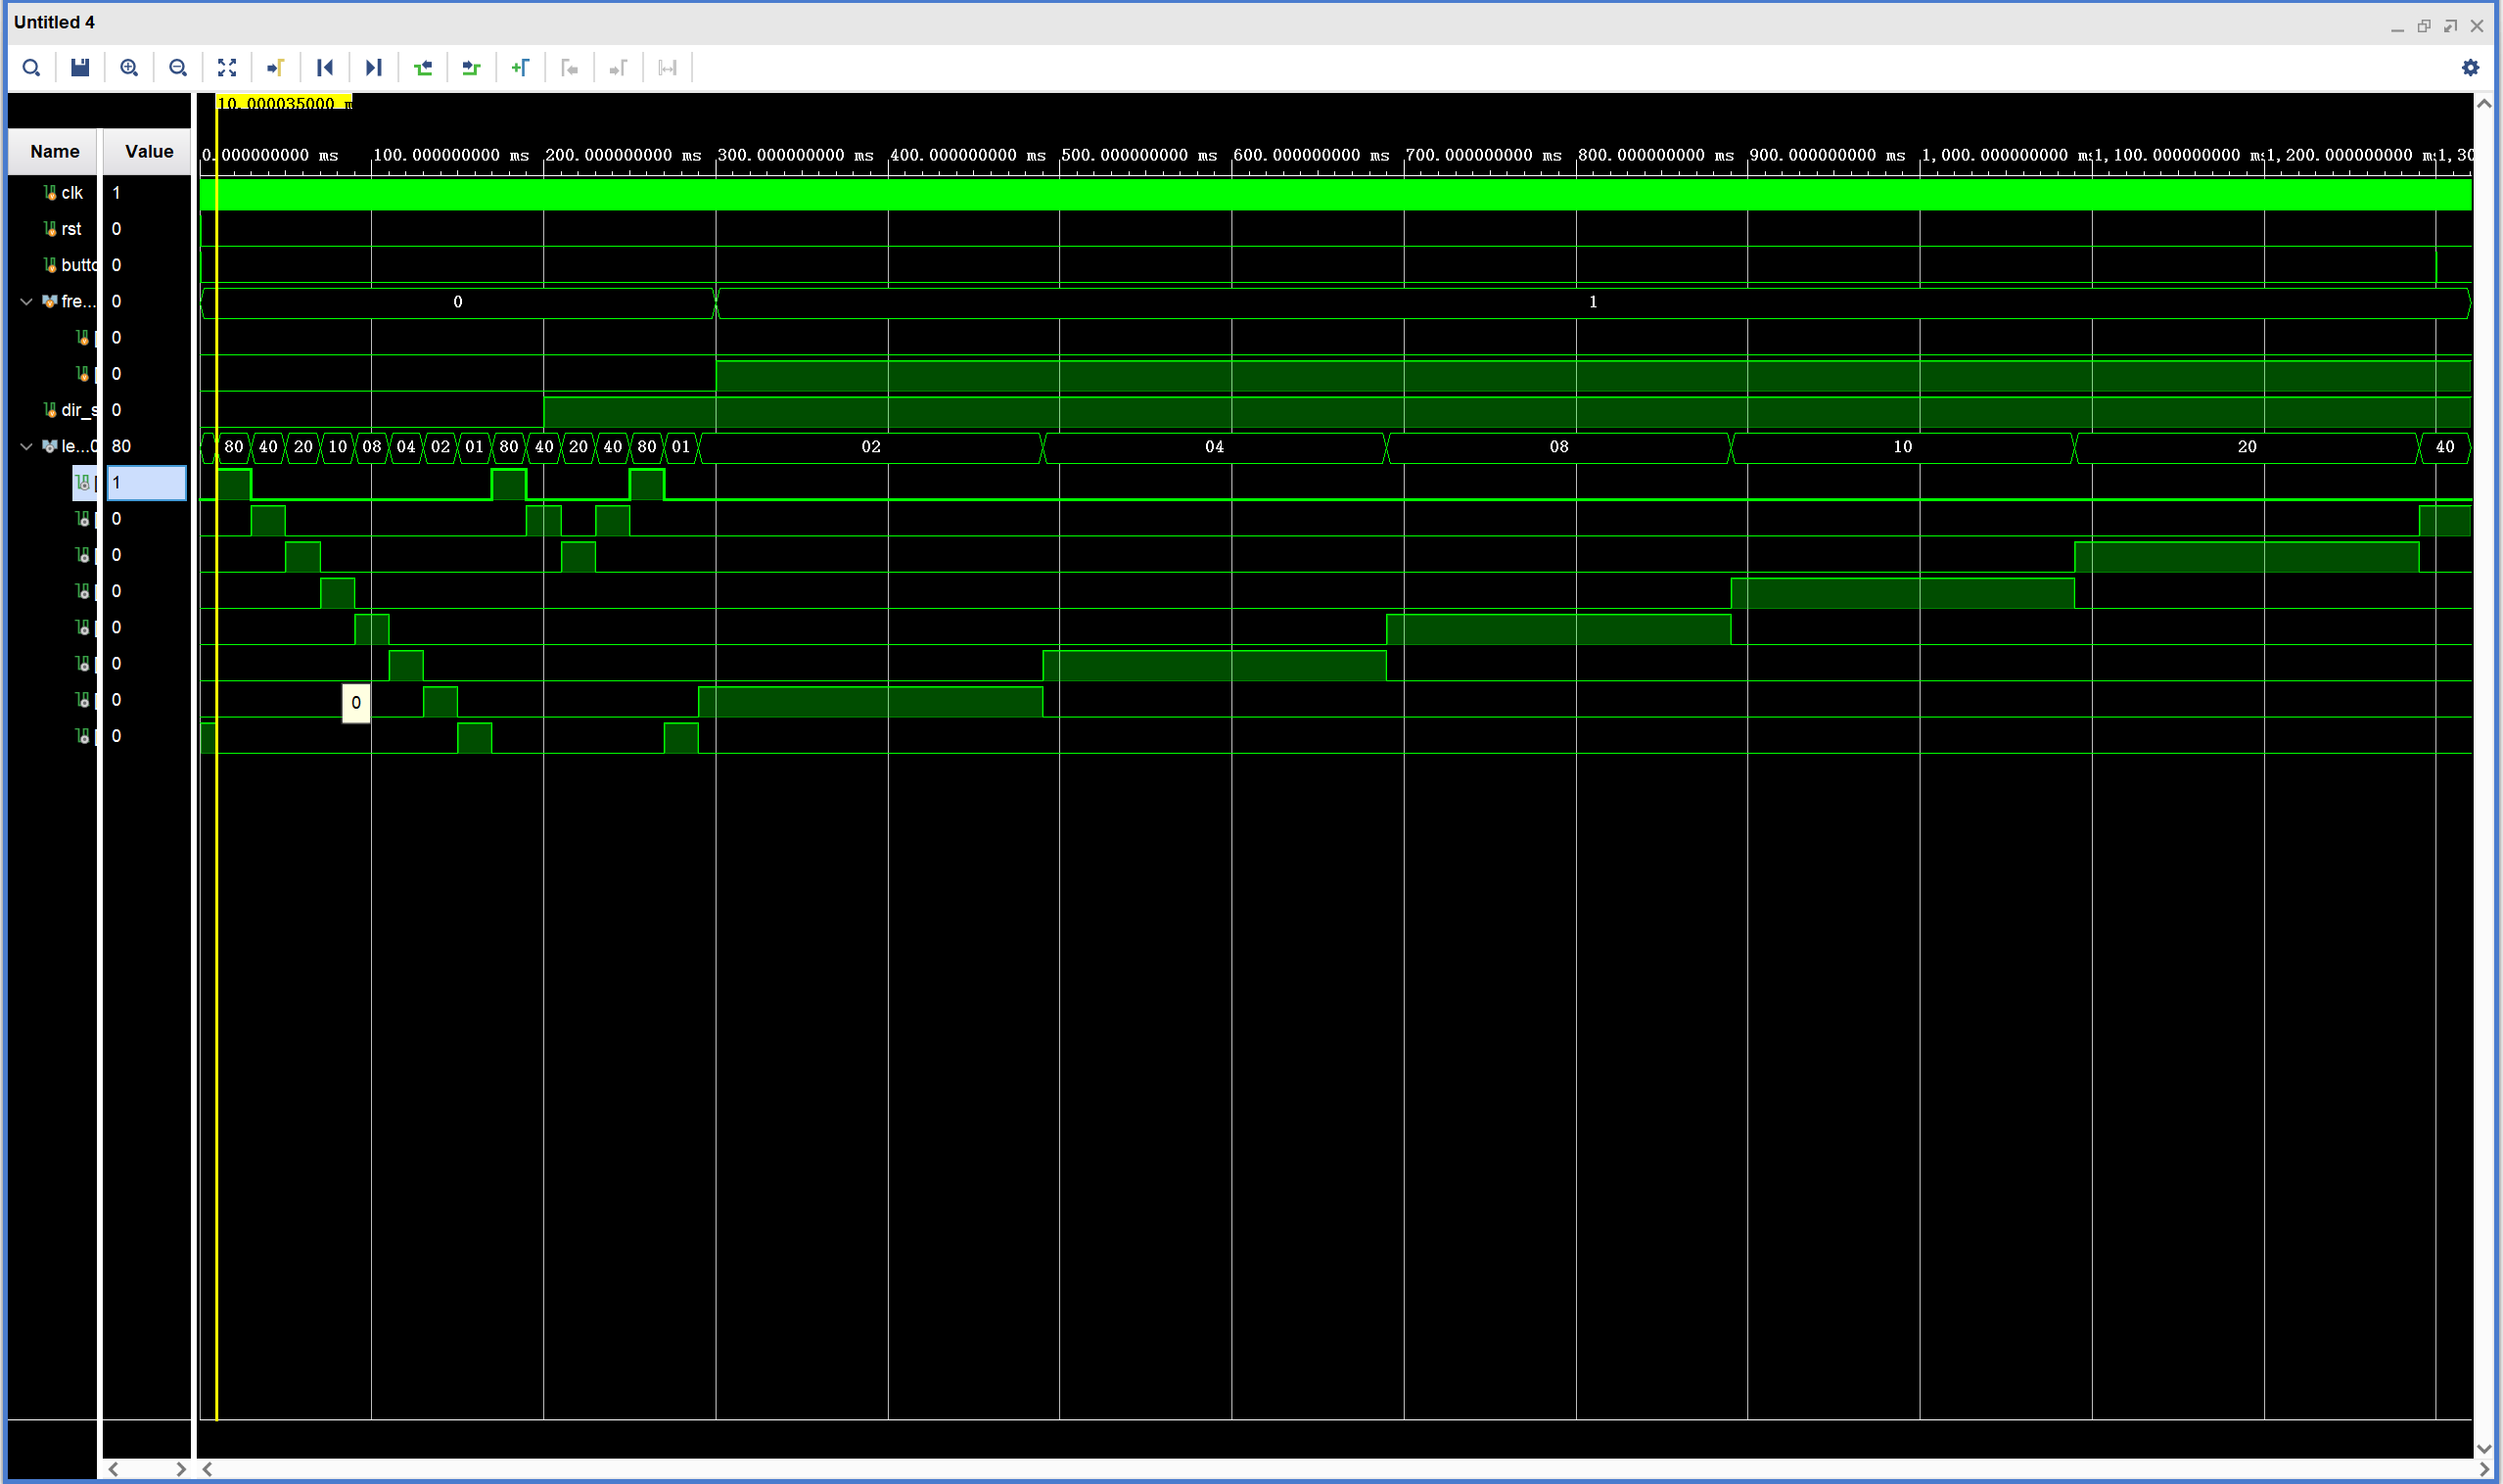
\includegraphics[width=0.8\textwidth]{1.png}\par
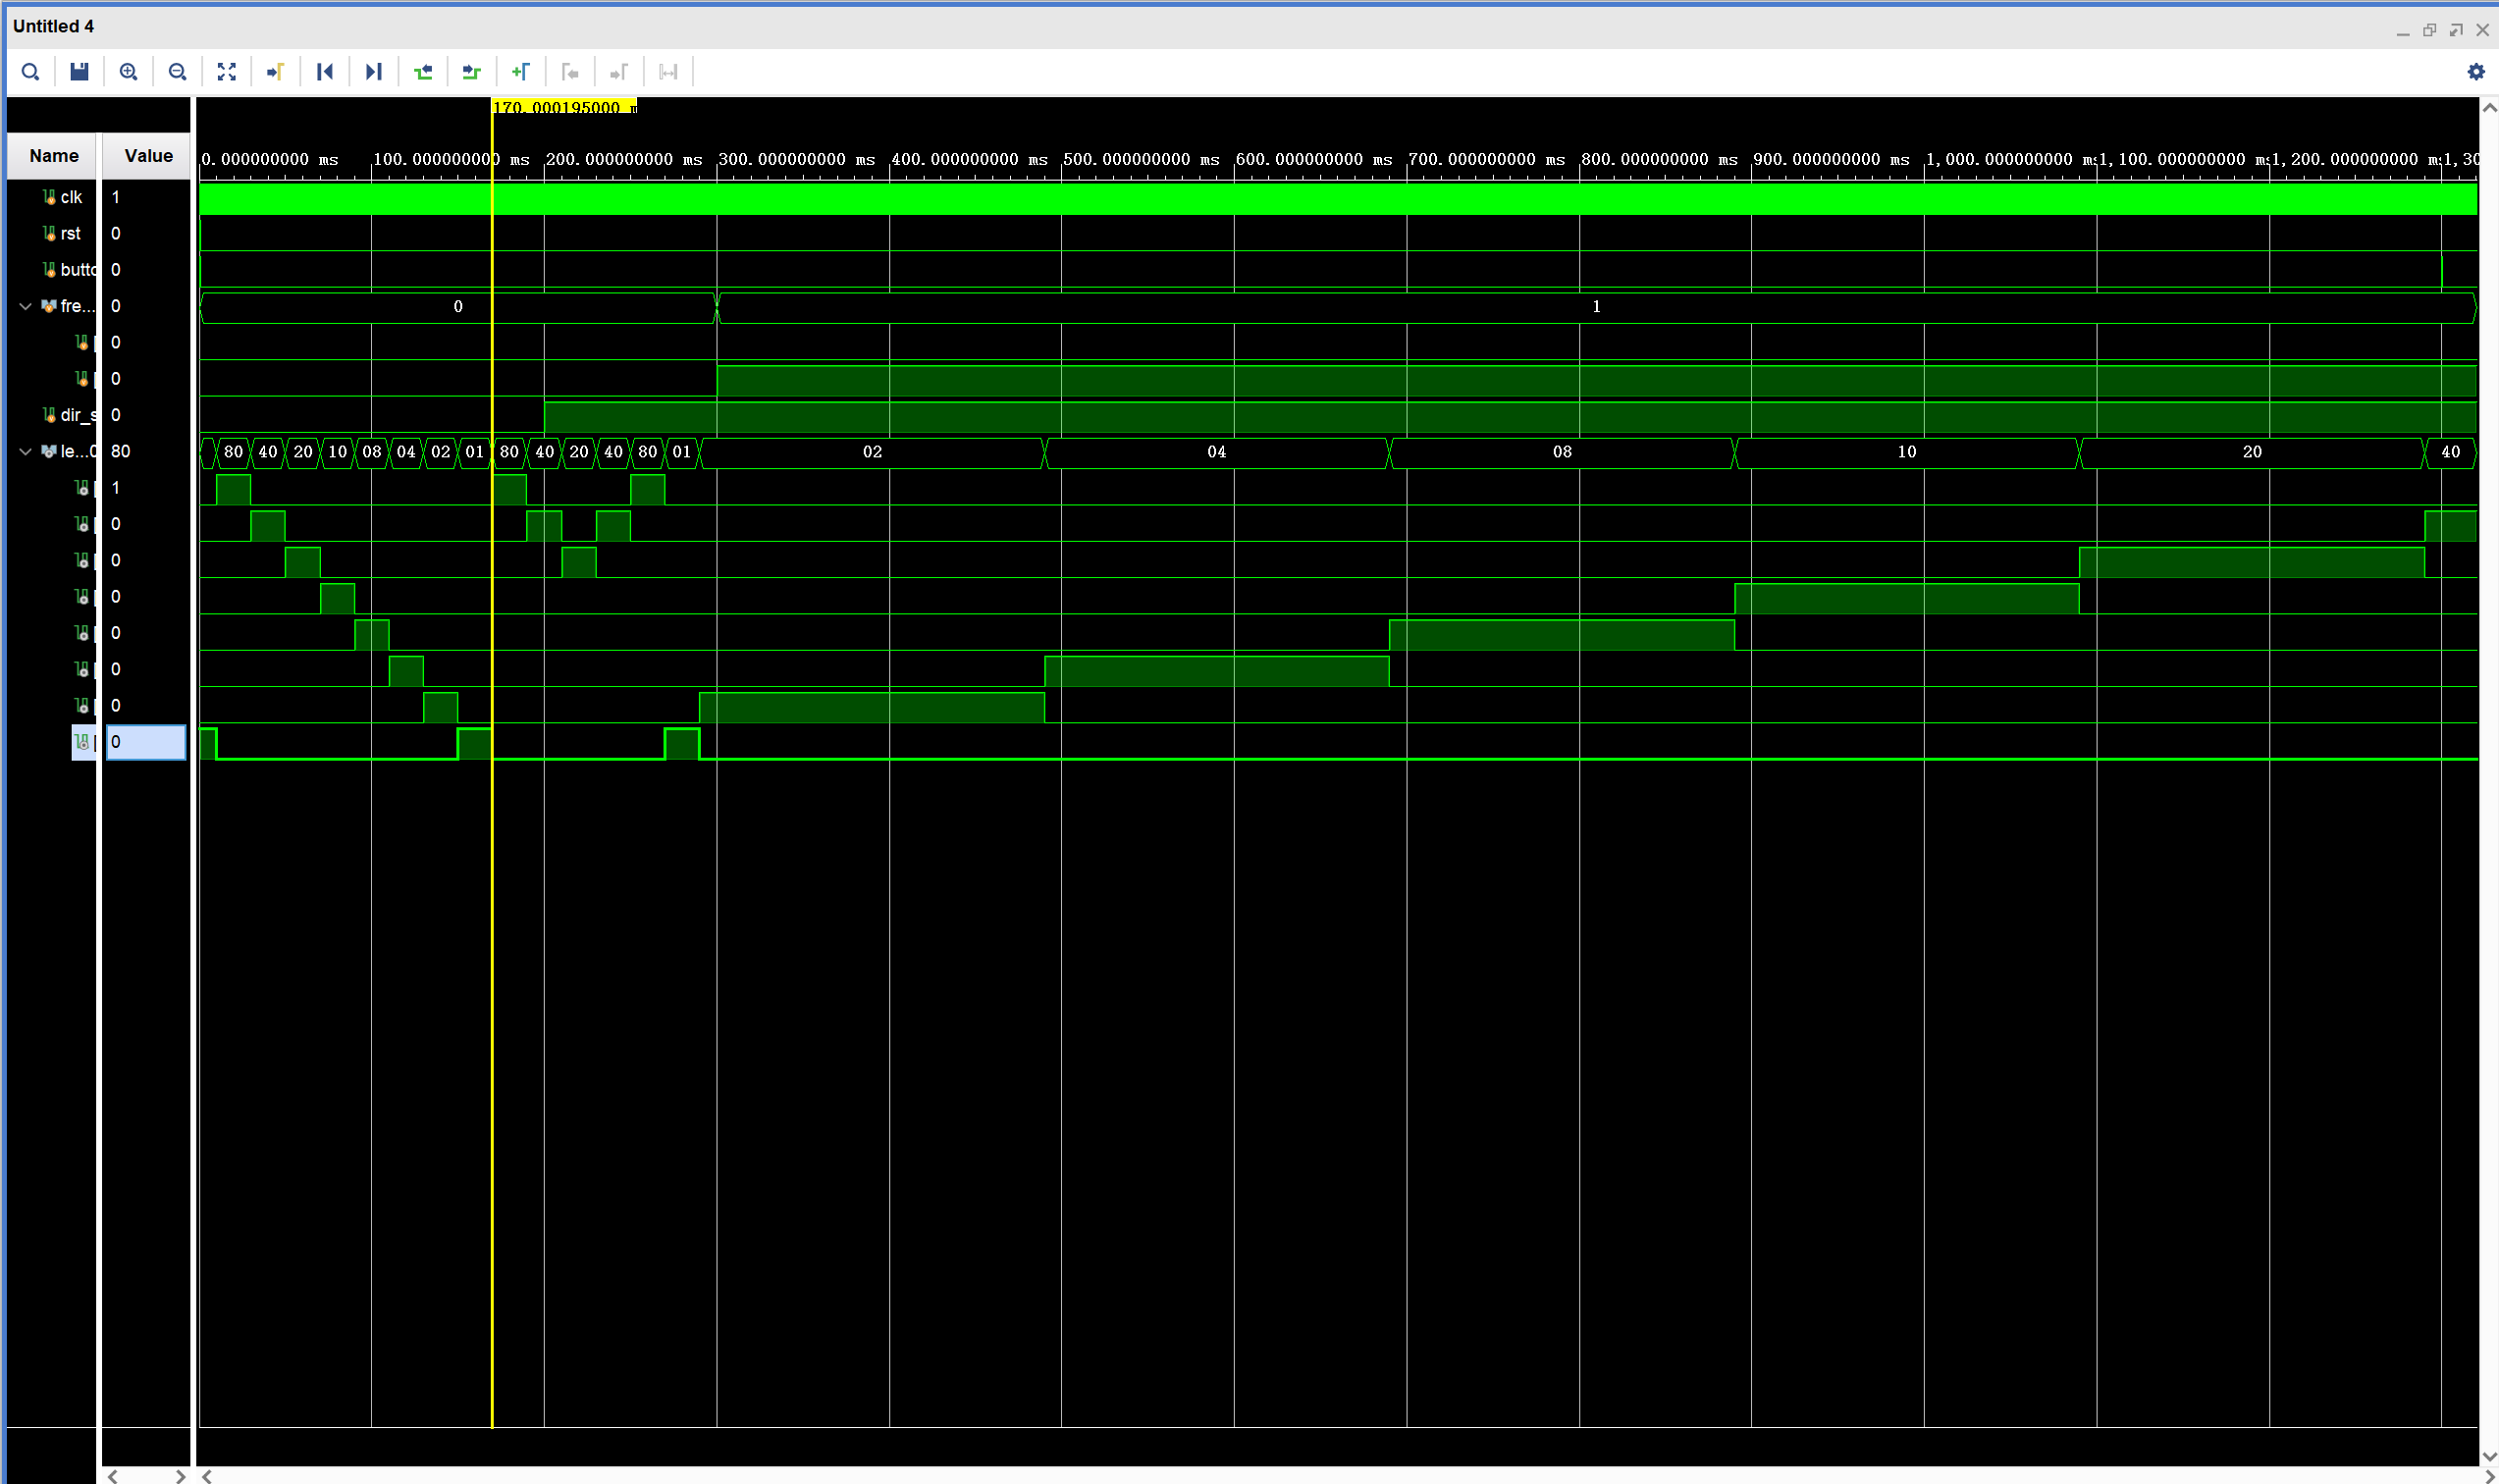
\includegraphics[width=0.8\textwidth]{2.png}\par
(1)流水灯初始复位,clr为1处于复位态,输出q一直为0。\par
(2)摁下启停按钮,流水灯准备启动\par
(3)设置频率为100Hz,间隔周期为0.01s\par
(4)流水灯从7向0依次亮起,周期性循环\par
(5)摁下方向按钮,灯亮起的方向改变,依旧进行周期性循环亮起\par
(6)改变频率为50Hz,灯亮起的间隔变为0.2s\par
(7)再次摁下启停按钮,流水灯停止循环亮起,亮的灯固定为最后一个\par





% 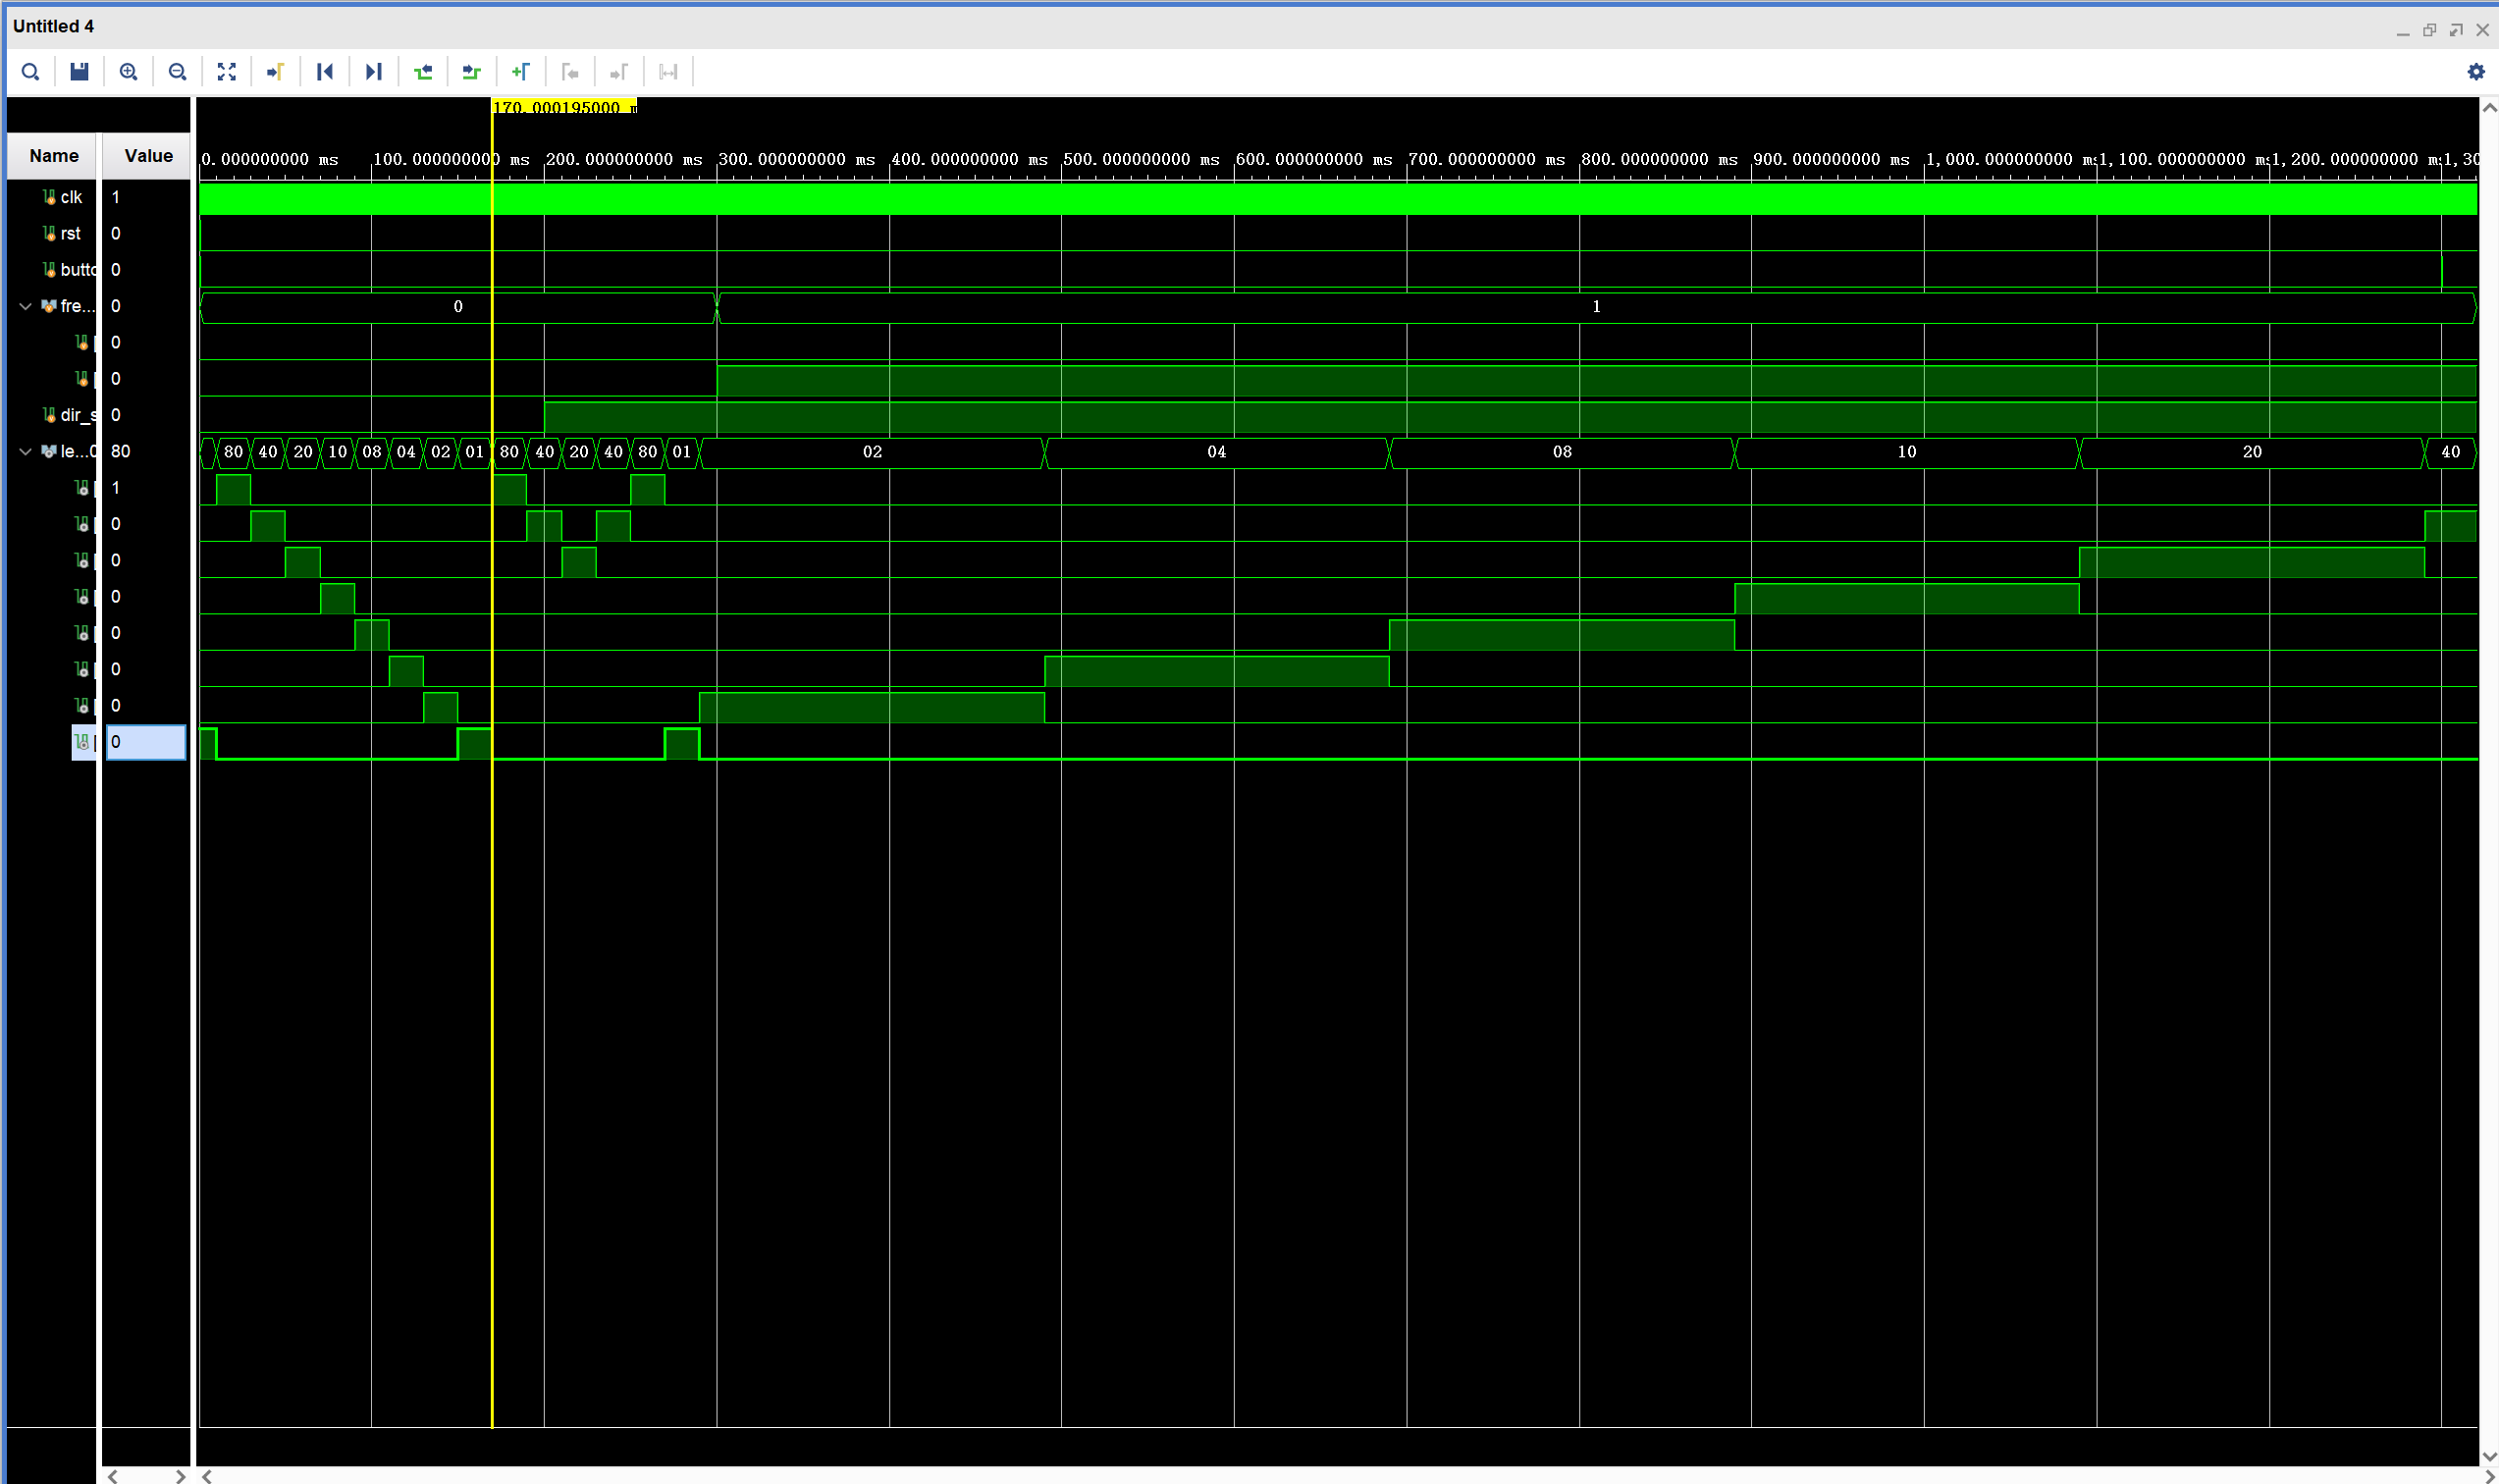
\includegraphics[width=0.8\textwidth]{2.png}\par
\section{RTL Analysis}
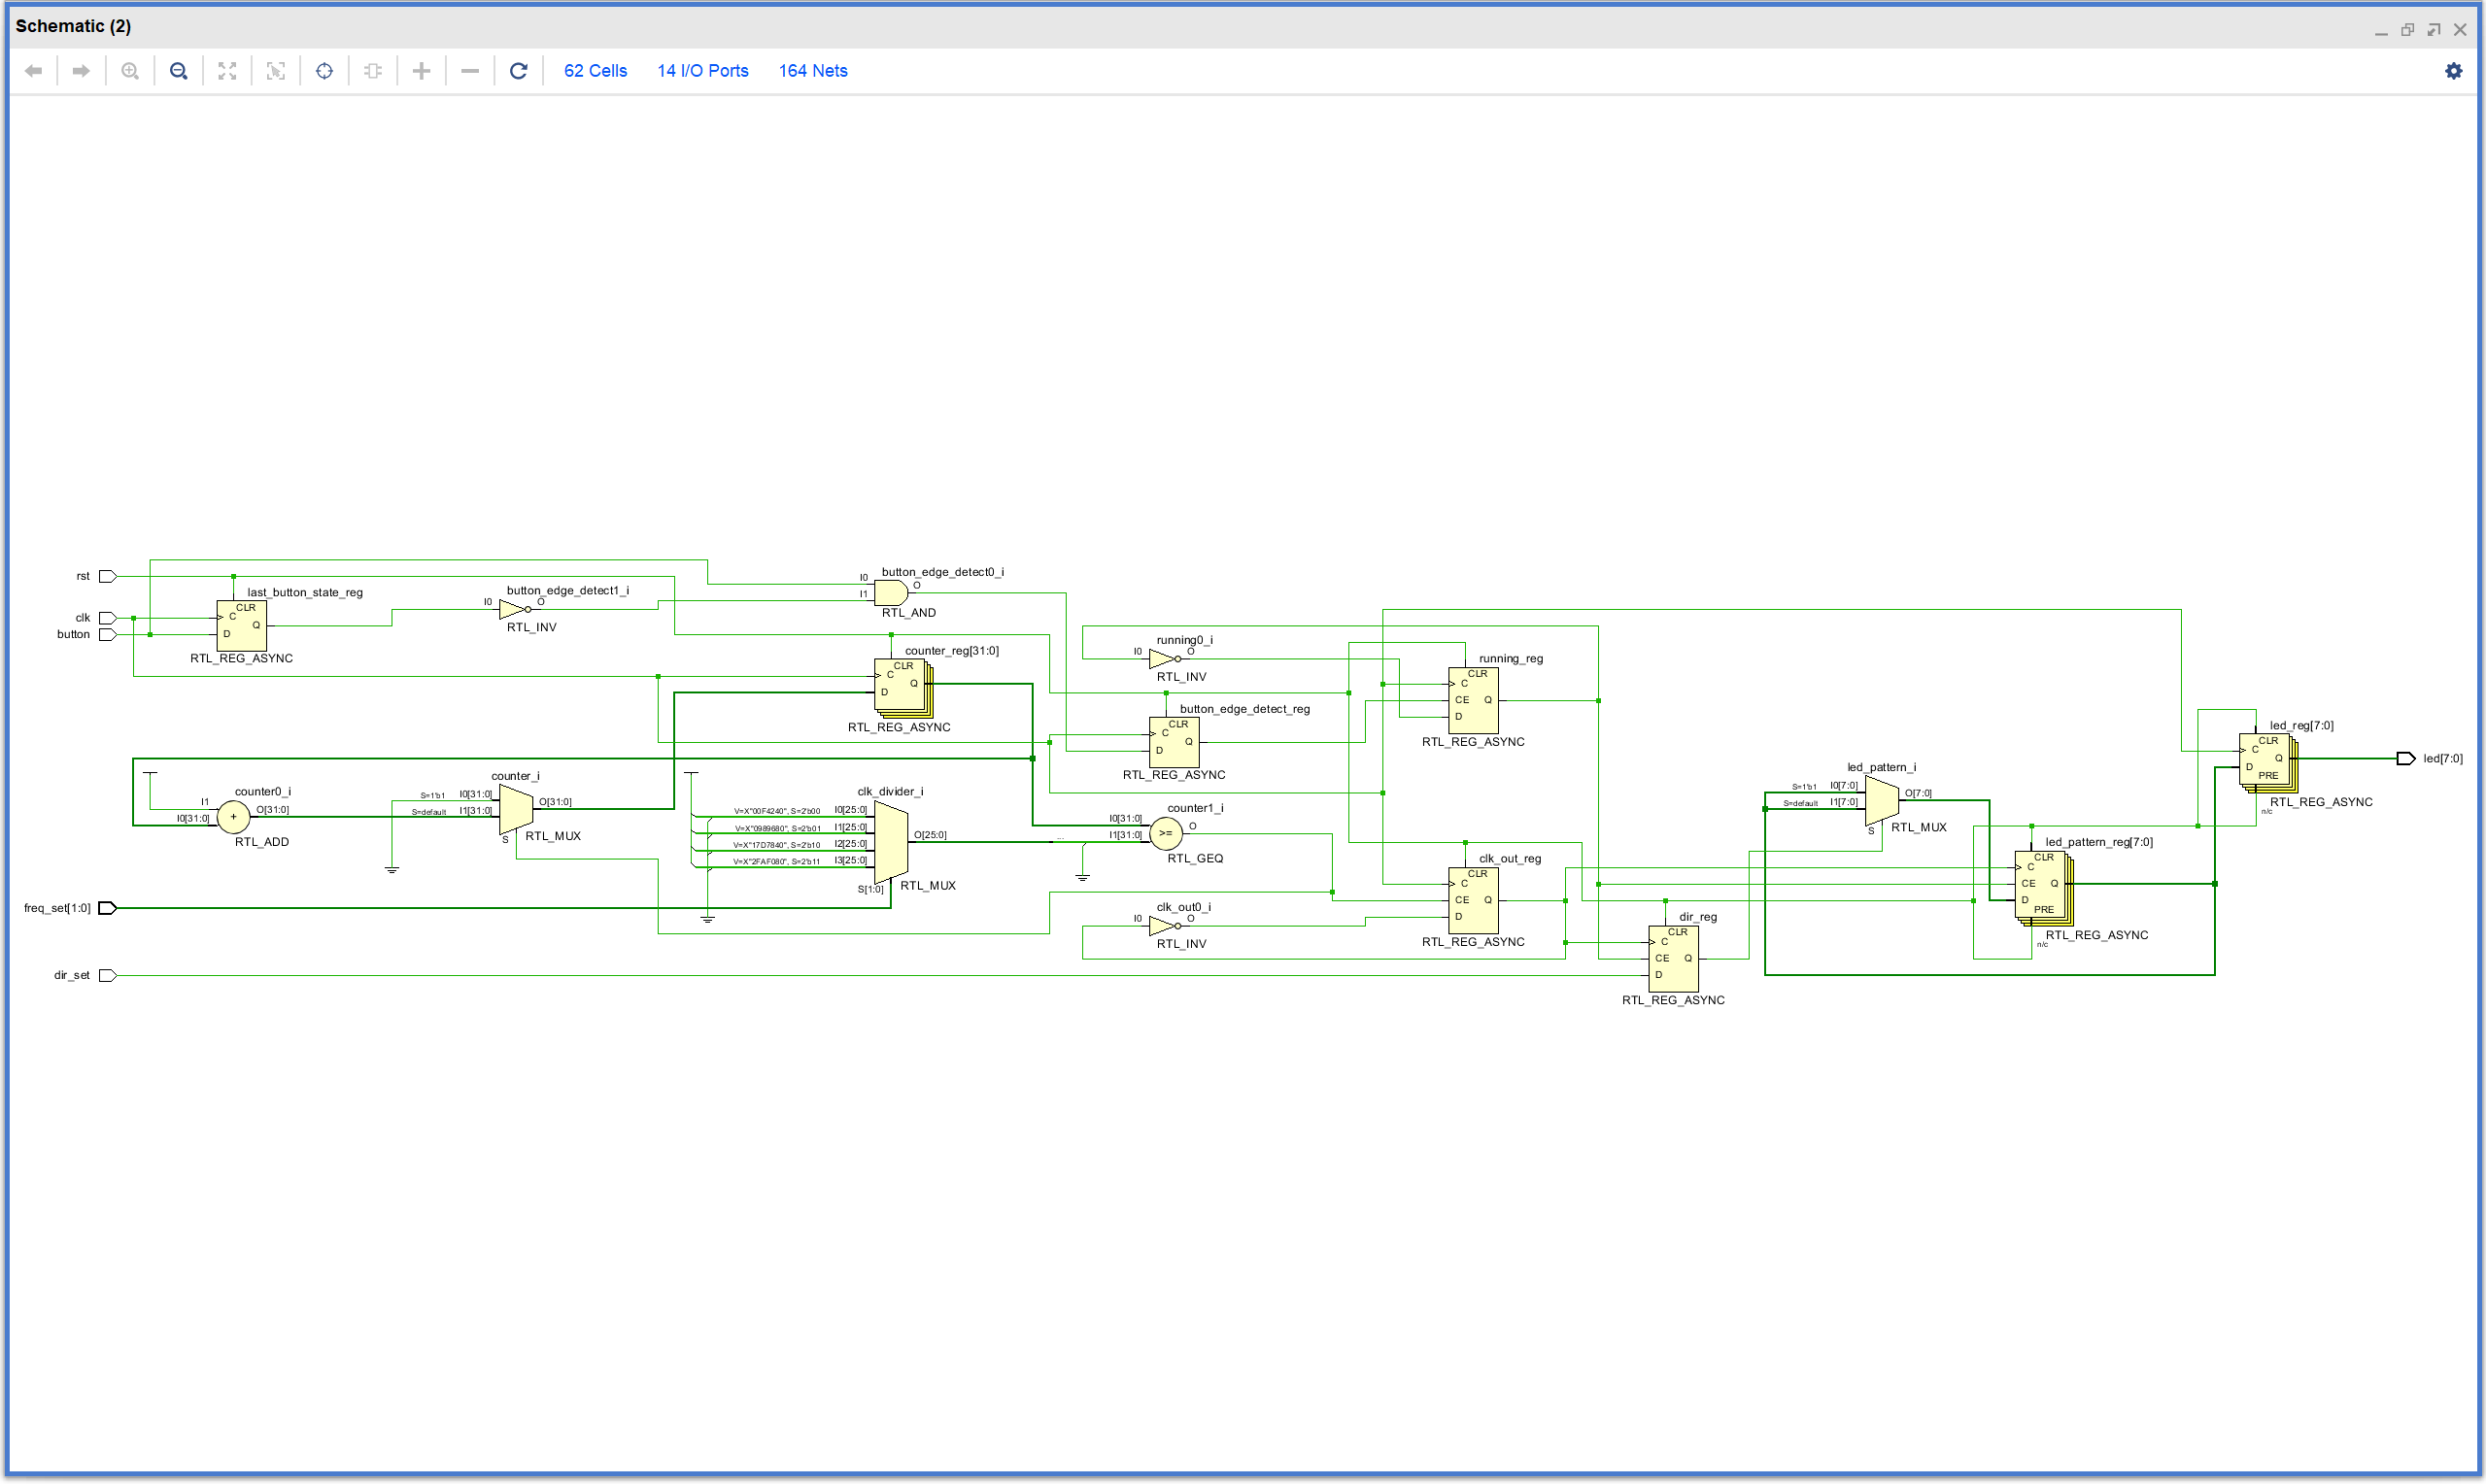
\includegraphics[width=0.8\textwidth]{3.png}\par
该图为RTL电路图,构成由计数器计时的流水灯电路。\par
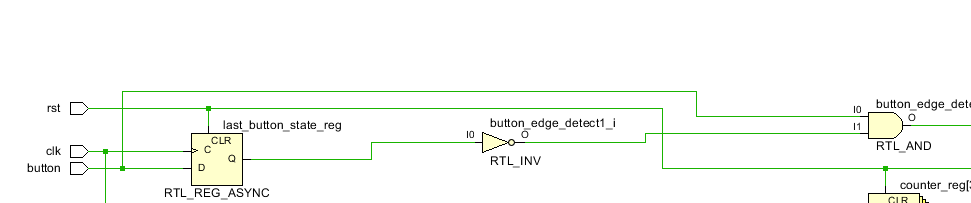
\includegraphics[width=0.8\textwidth]{4.png}\par
该图为电路中的边沿检测寄存器级联的位置。\par


\section{计数器最大值计算}
计数器最大值=时间间隔×时钟频率\par
0.01秒对应的计数增加:1,000,000\par
0.1秒对应的计数增加:10,000,000\par
0.25秒对应的计数增加:25,000,000\par
0.5秒对应的计数增加:50,000,000\par
$$
$$
% 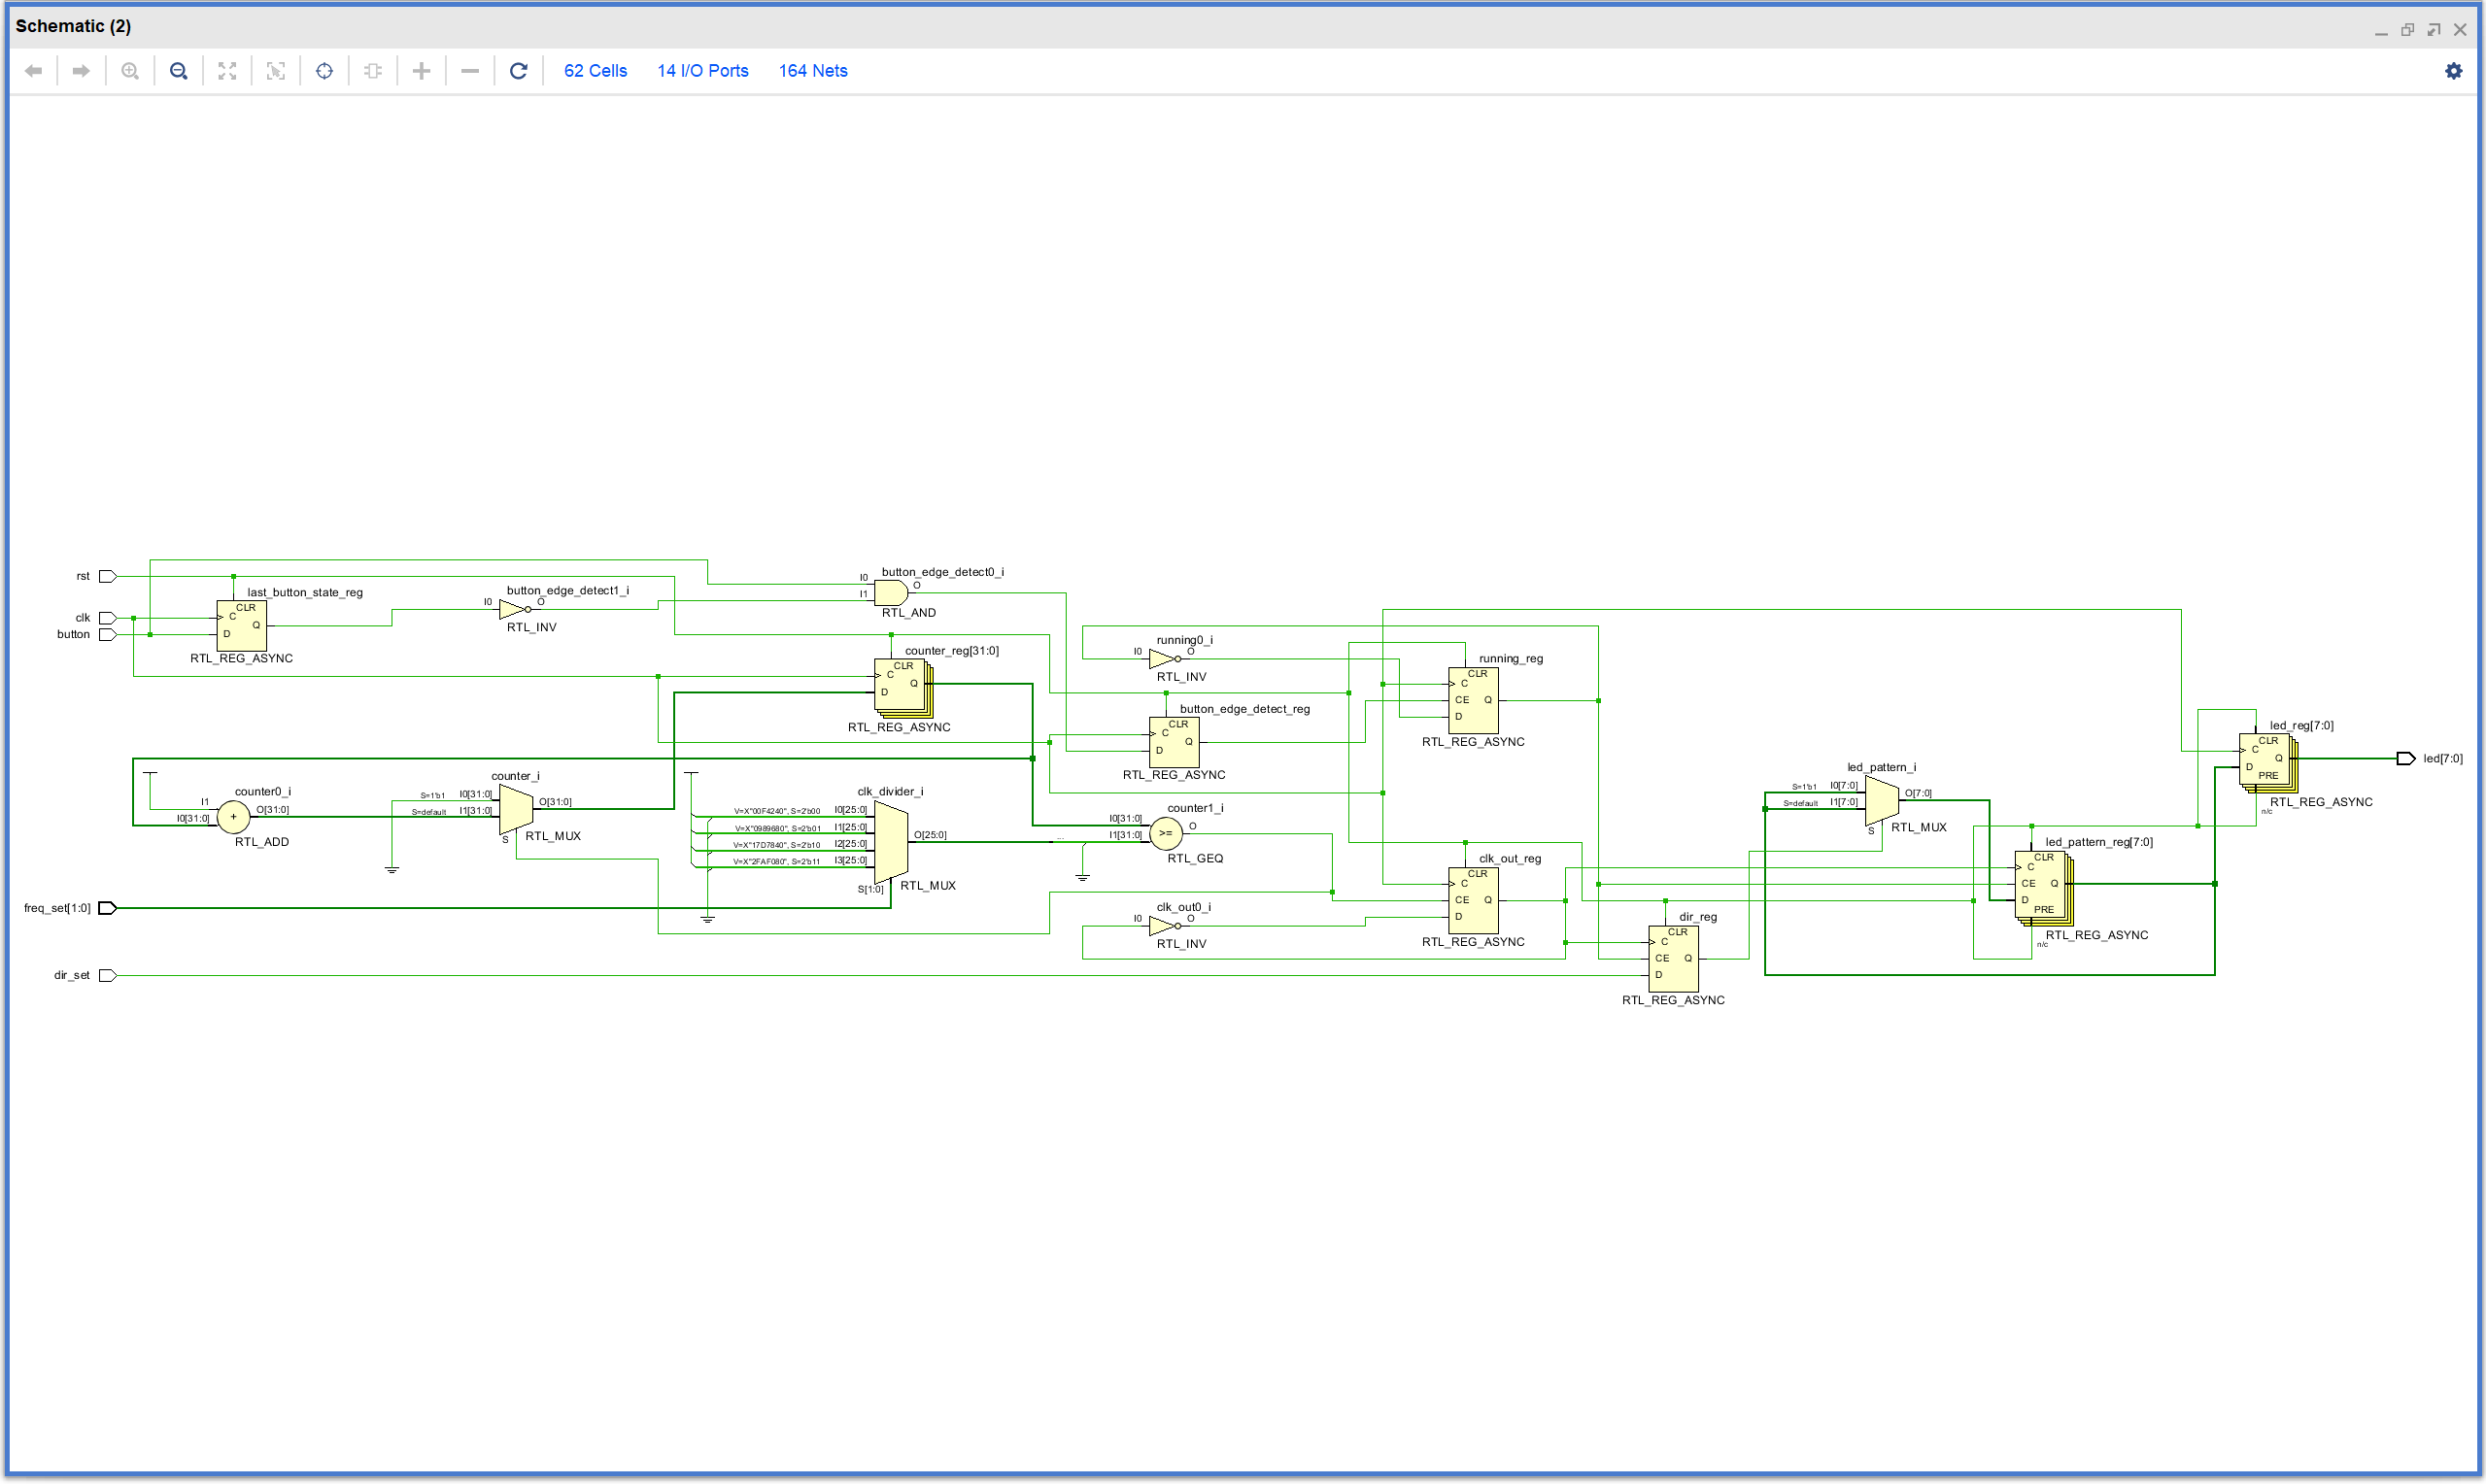
\includegraphics[width=0.8\textwidth]{3.png}\par
Synthesis schematic\par


% \section{阻塞}
% 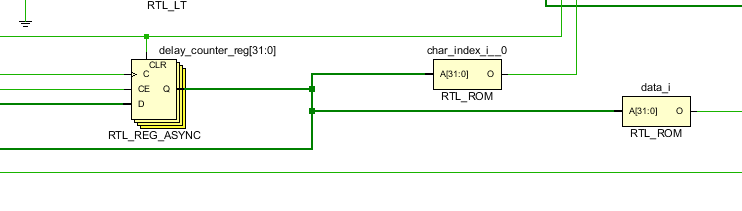
\includegraphics[width=0.8\textwidth]{11.png}\par
% 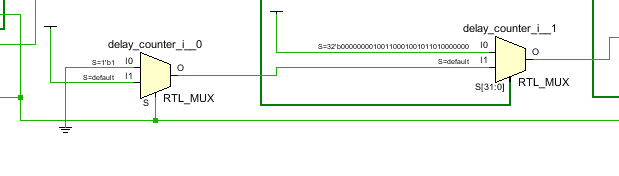
\includegraphics[width=0.8\textwidth]{12.png}\par
% 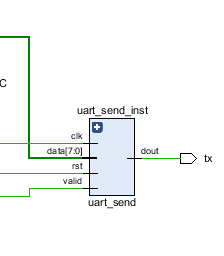
\includegraphics[width=0.8\textwidth]{13.png}\par
% \section{无阻塞}
% 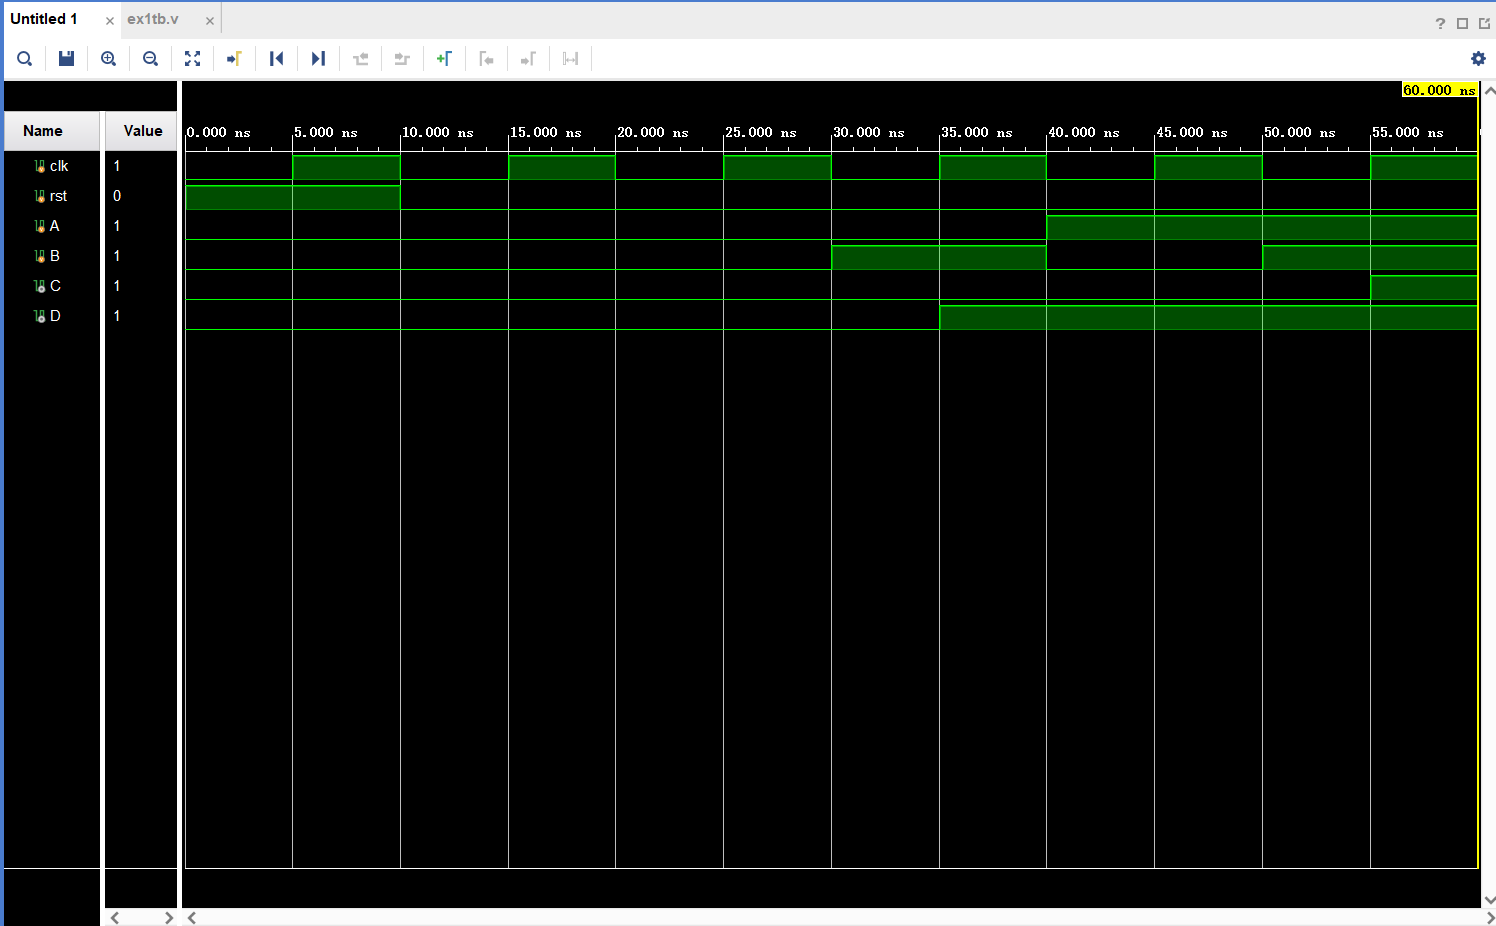
\includegraphics[width=0.8\textwidth]{21.png}\par
% 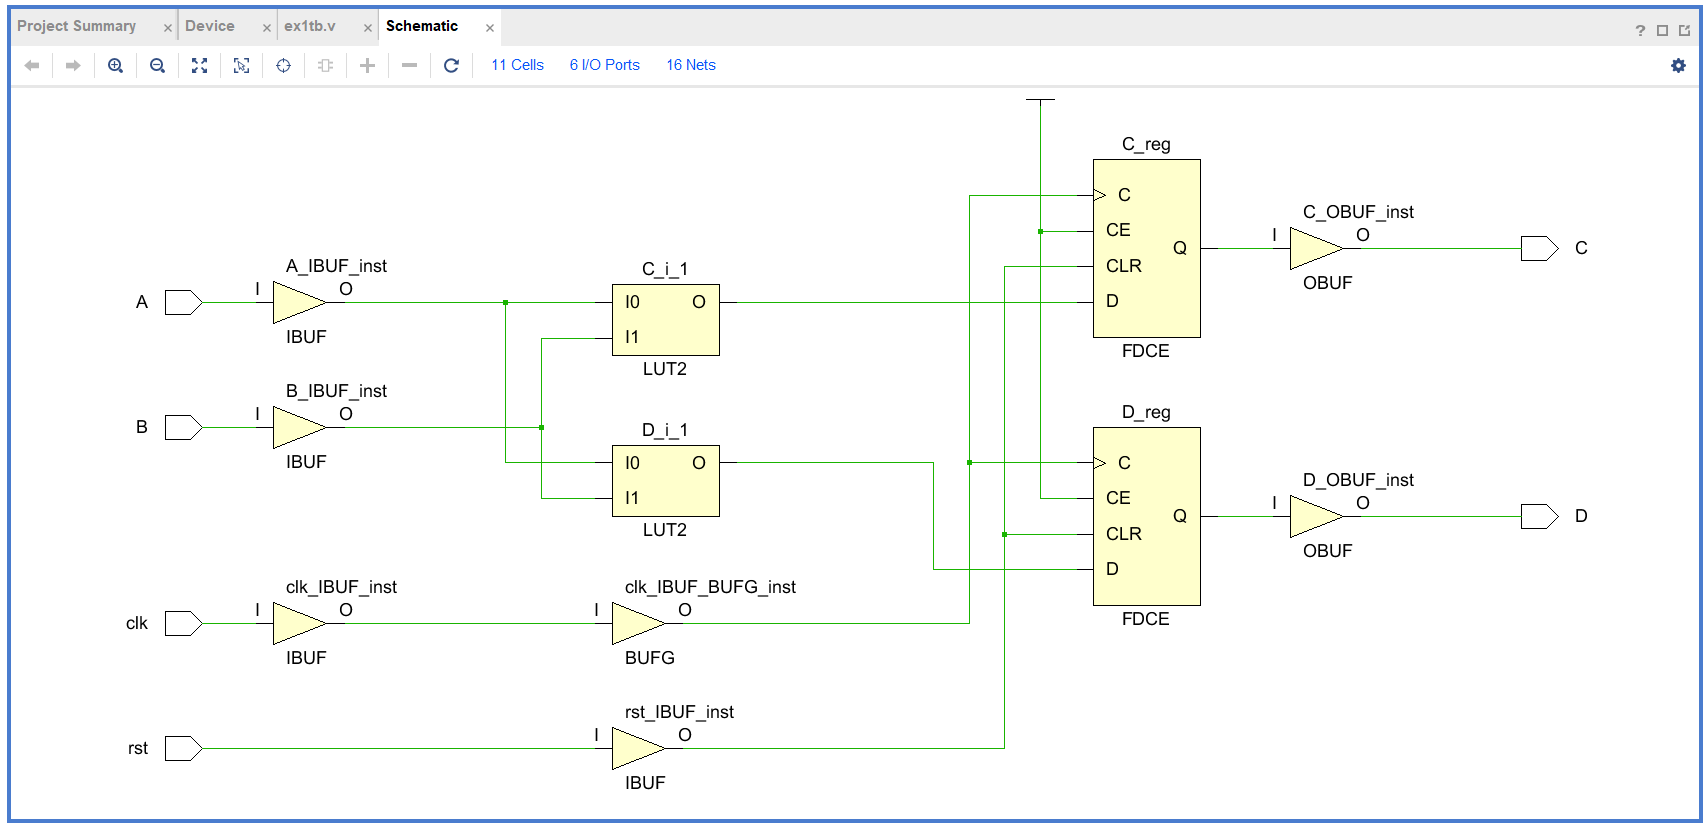
\includegraphics[width=0.8\textwidth]{22.png}\par
% 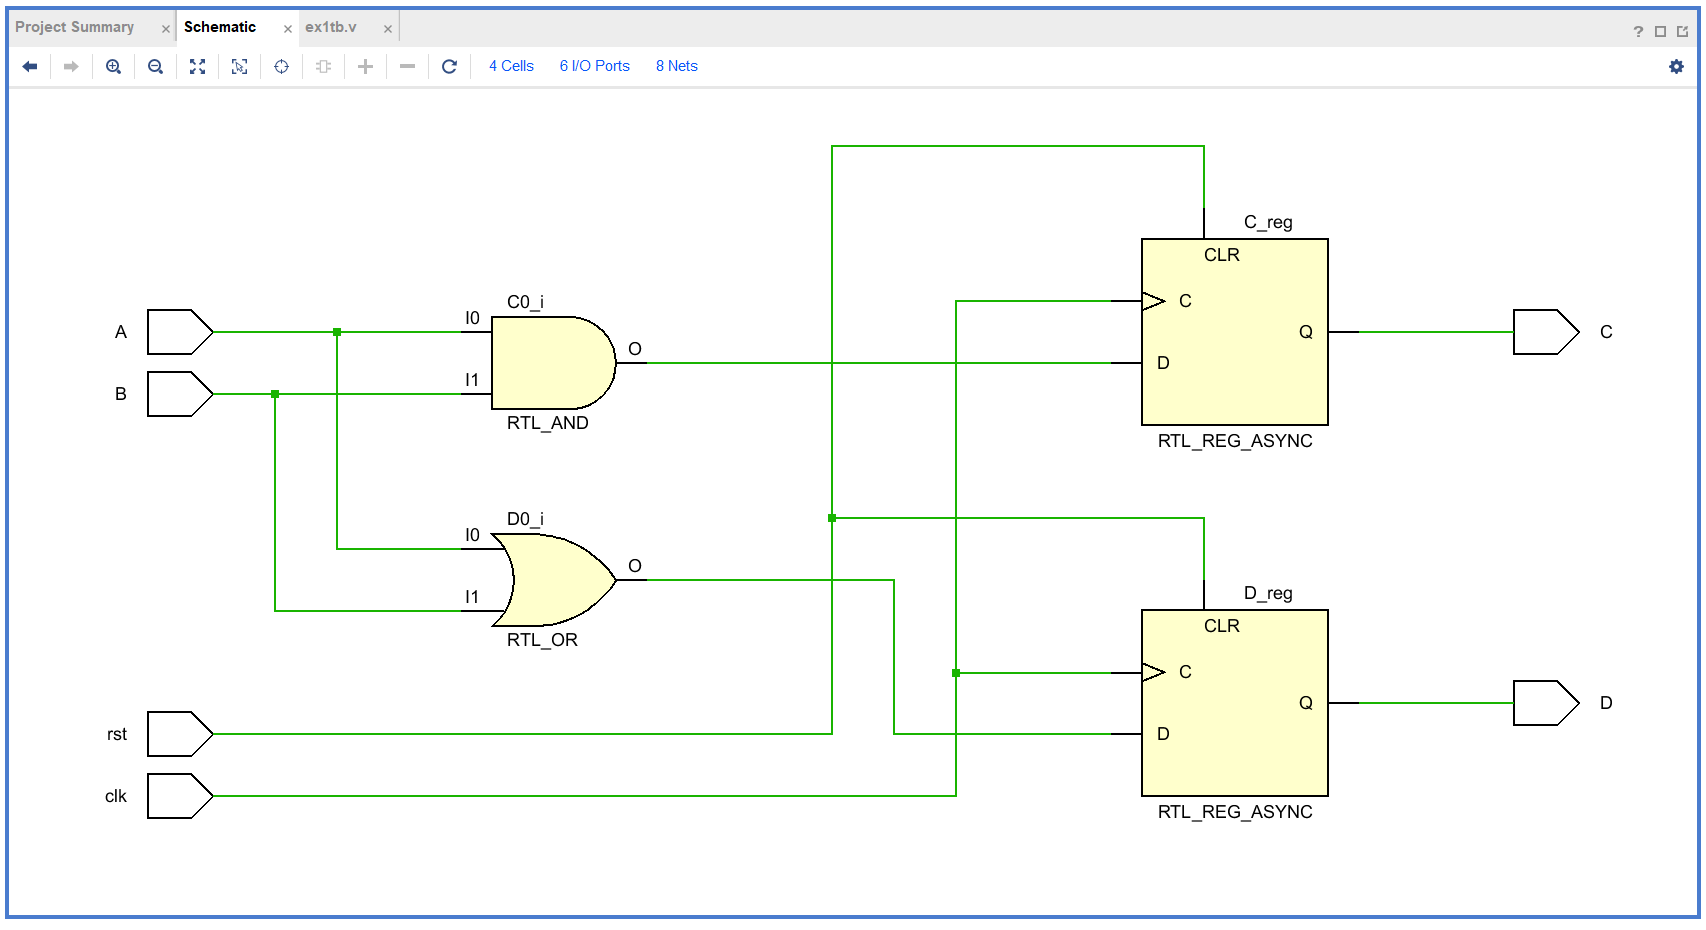
\includegraphics[width=0.8\textwidth]{23.png}\par
\section{课后作业}
对比1\par
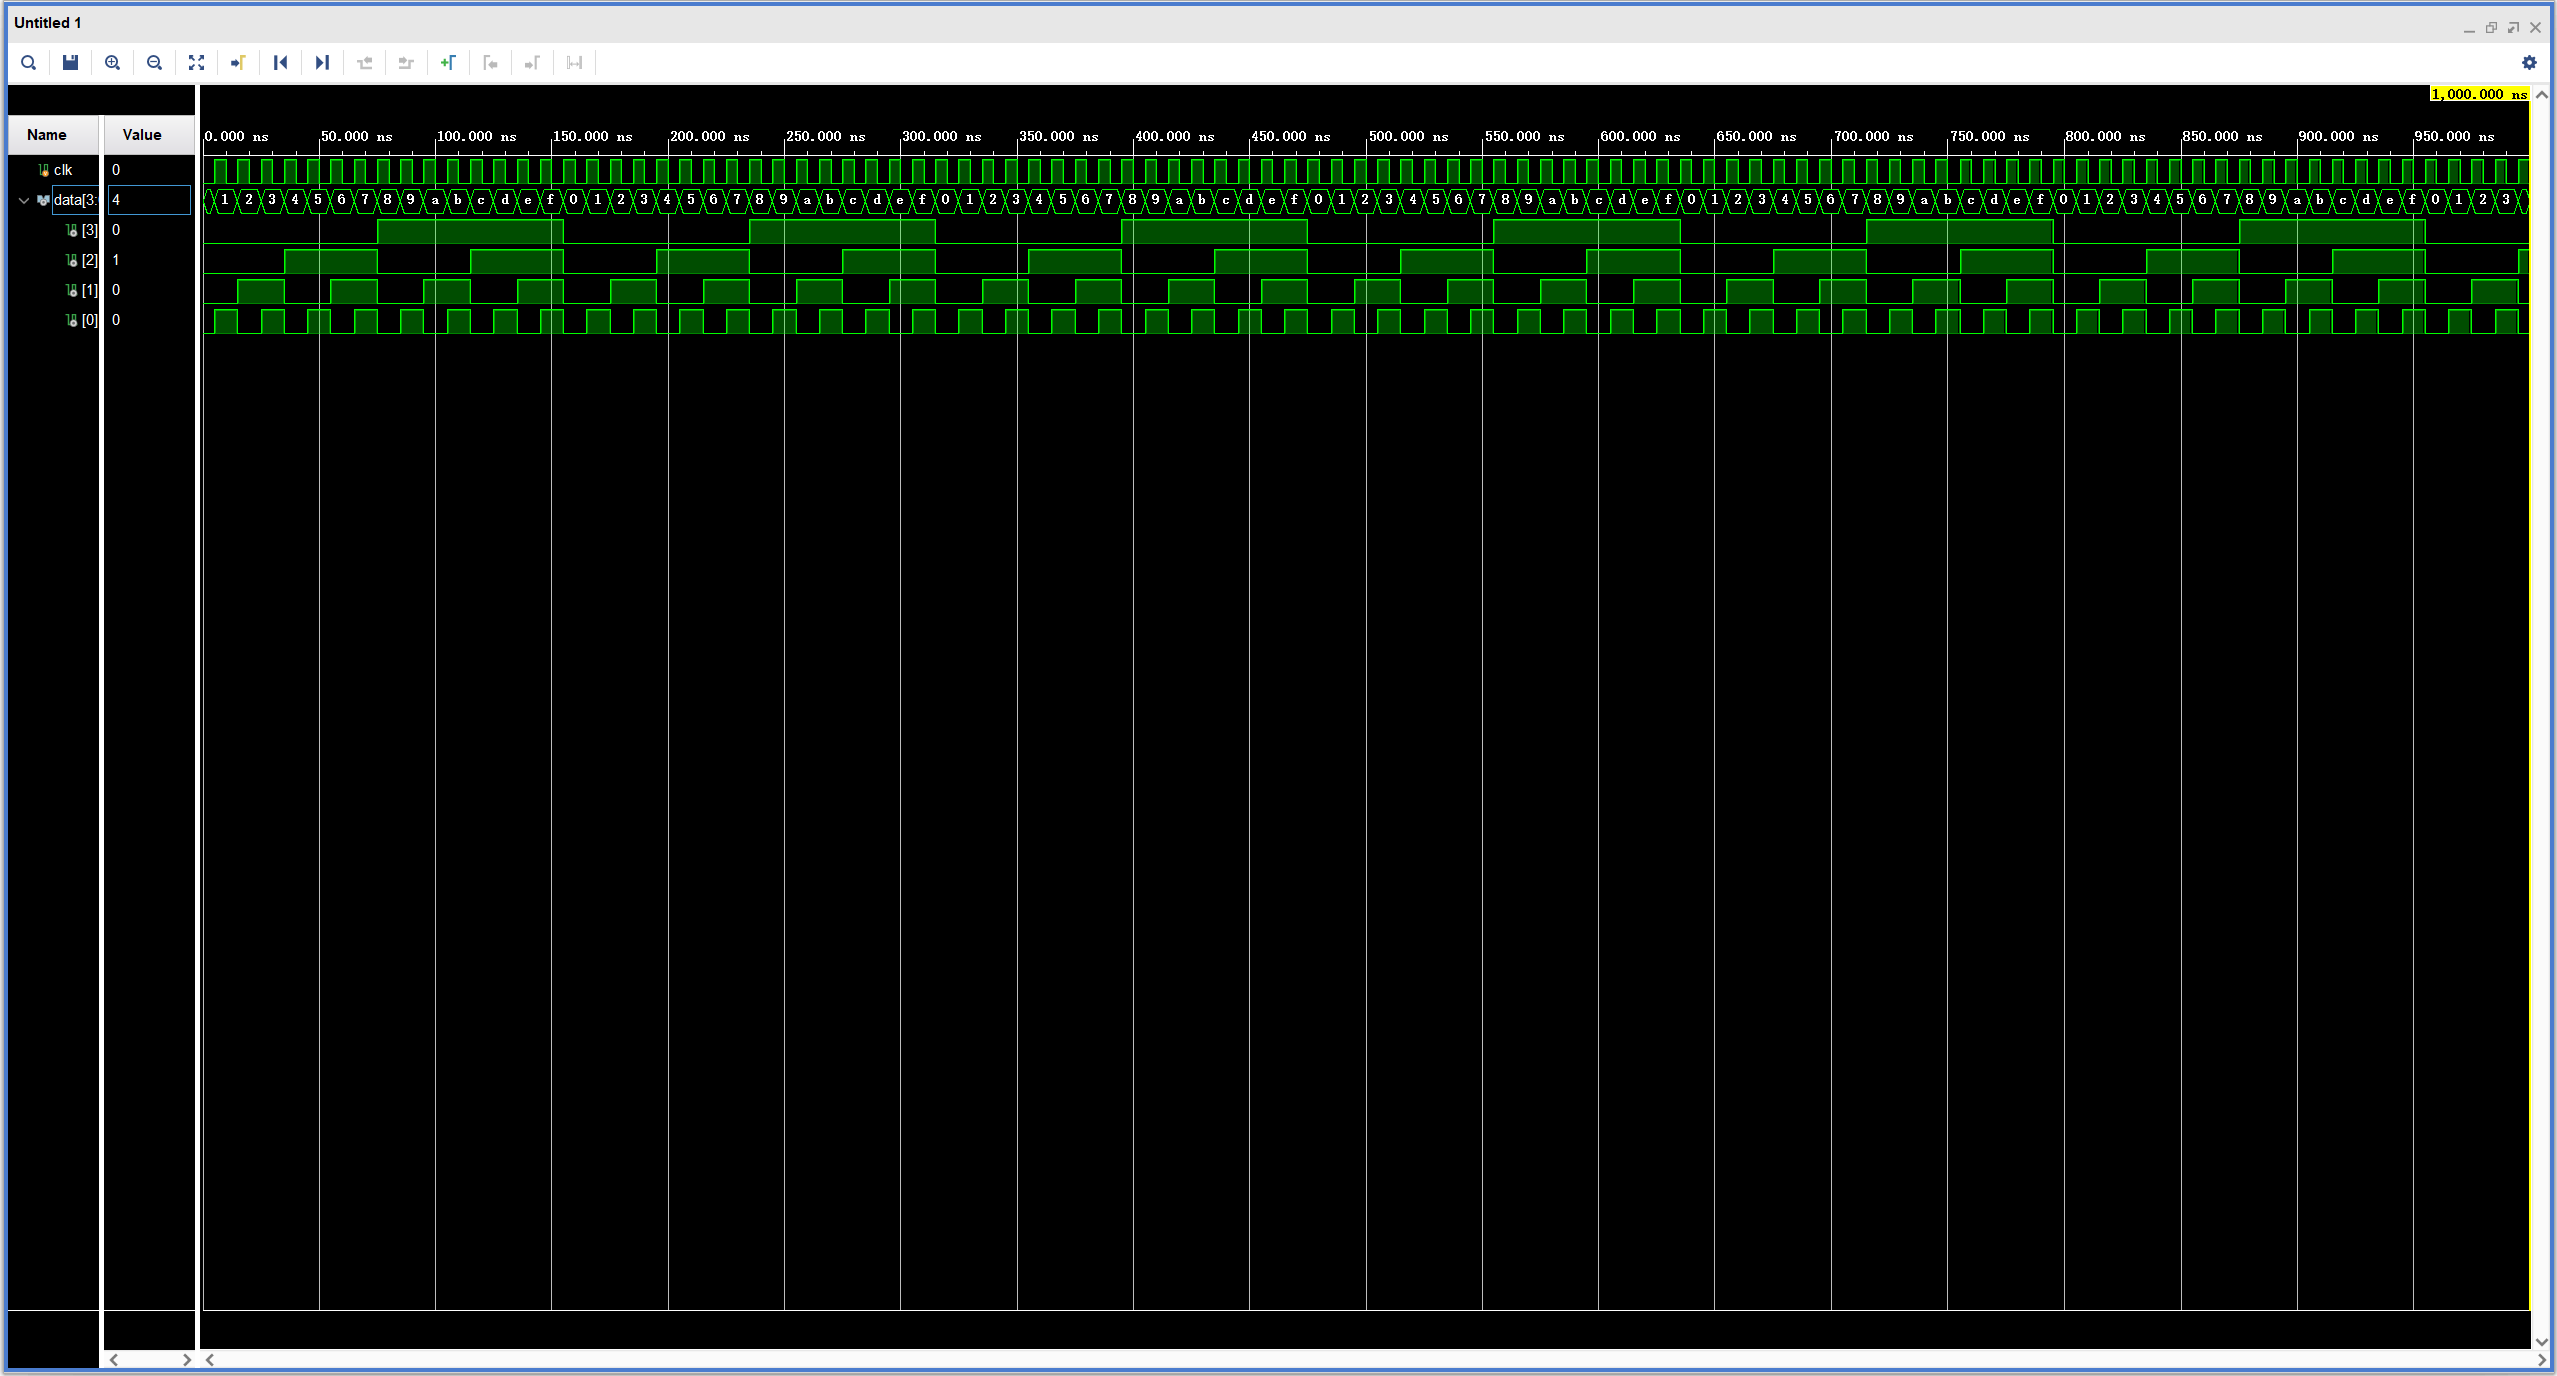
\includegraphics[width=0.3\textwidth]{nonex11.png}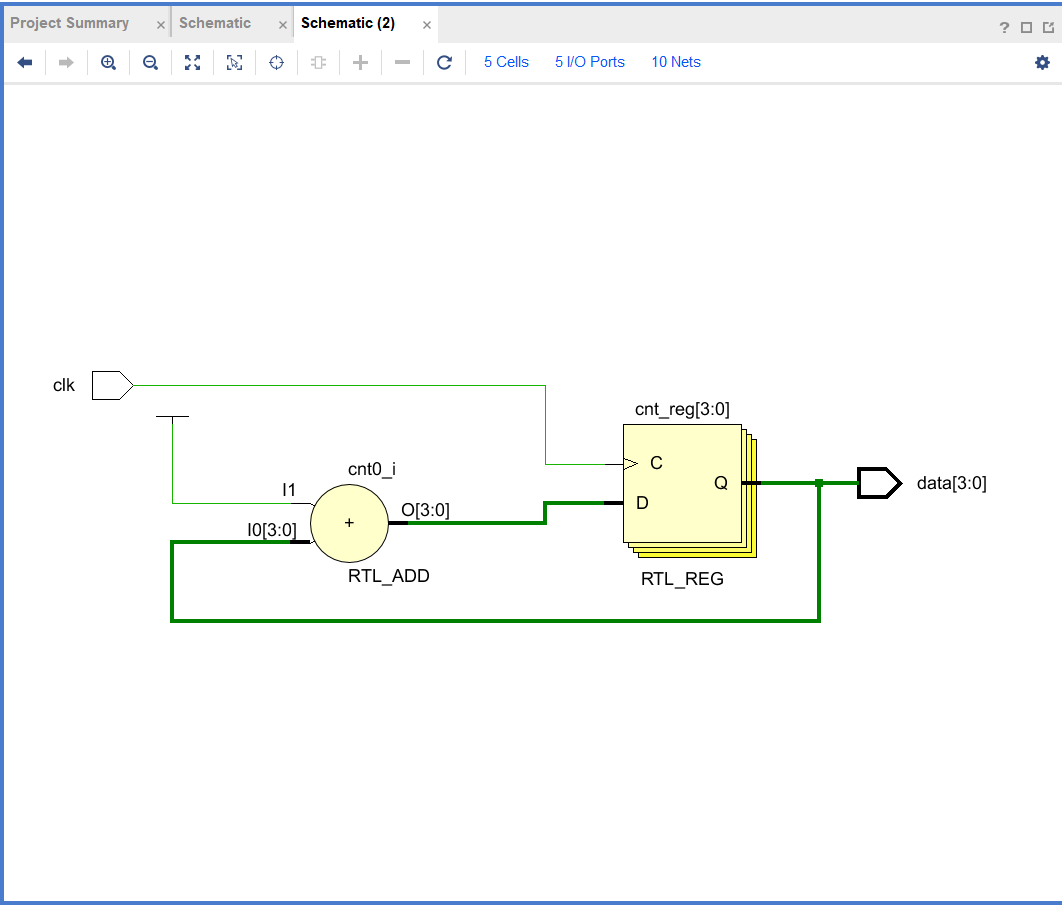
\includegraphics[width=0.3\textwidth]{nonex12.png}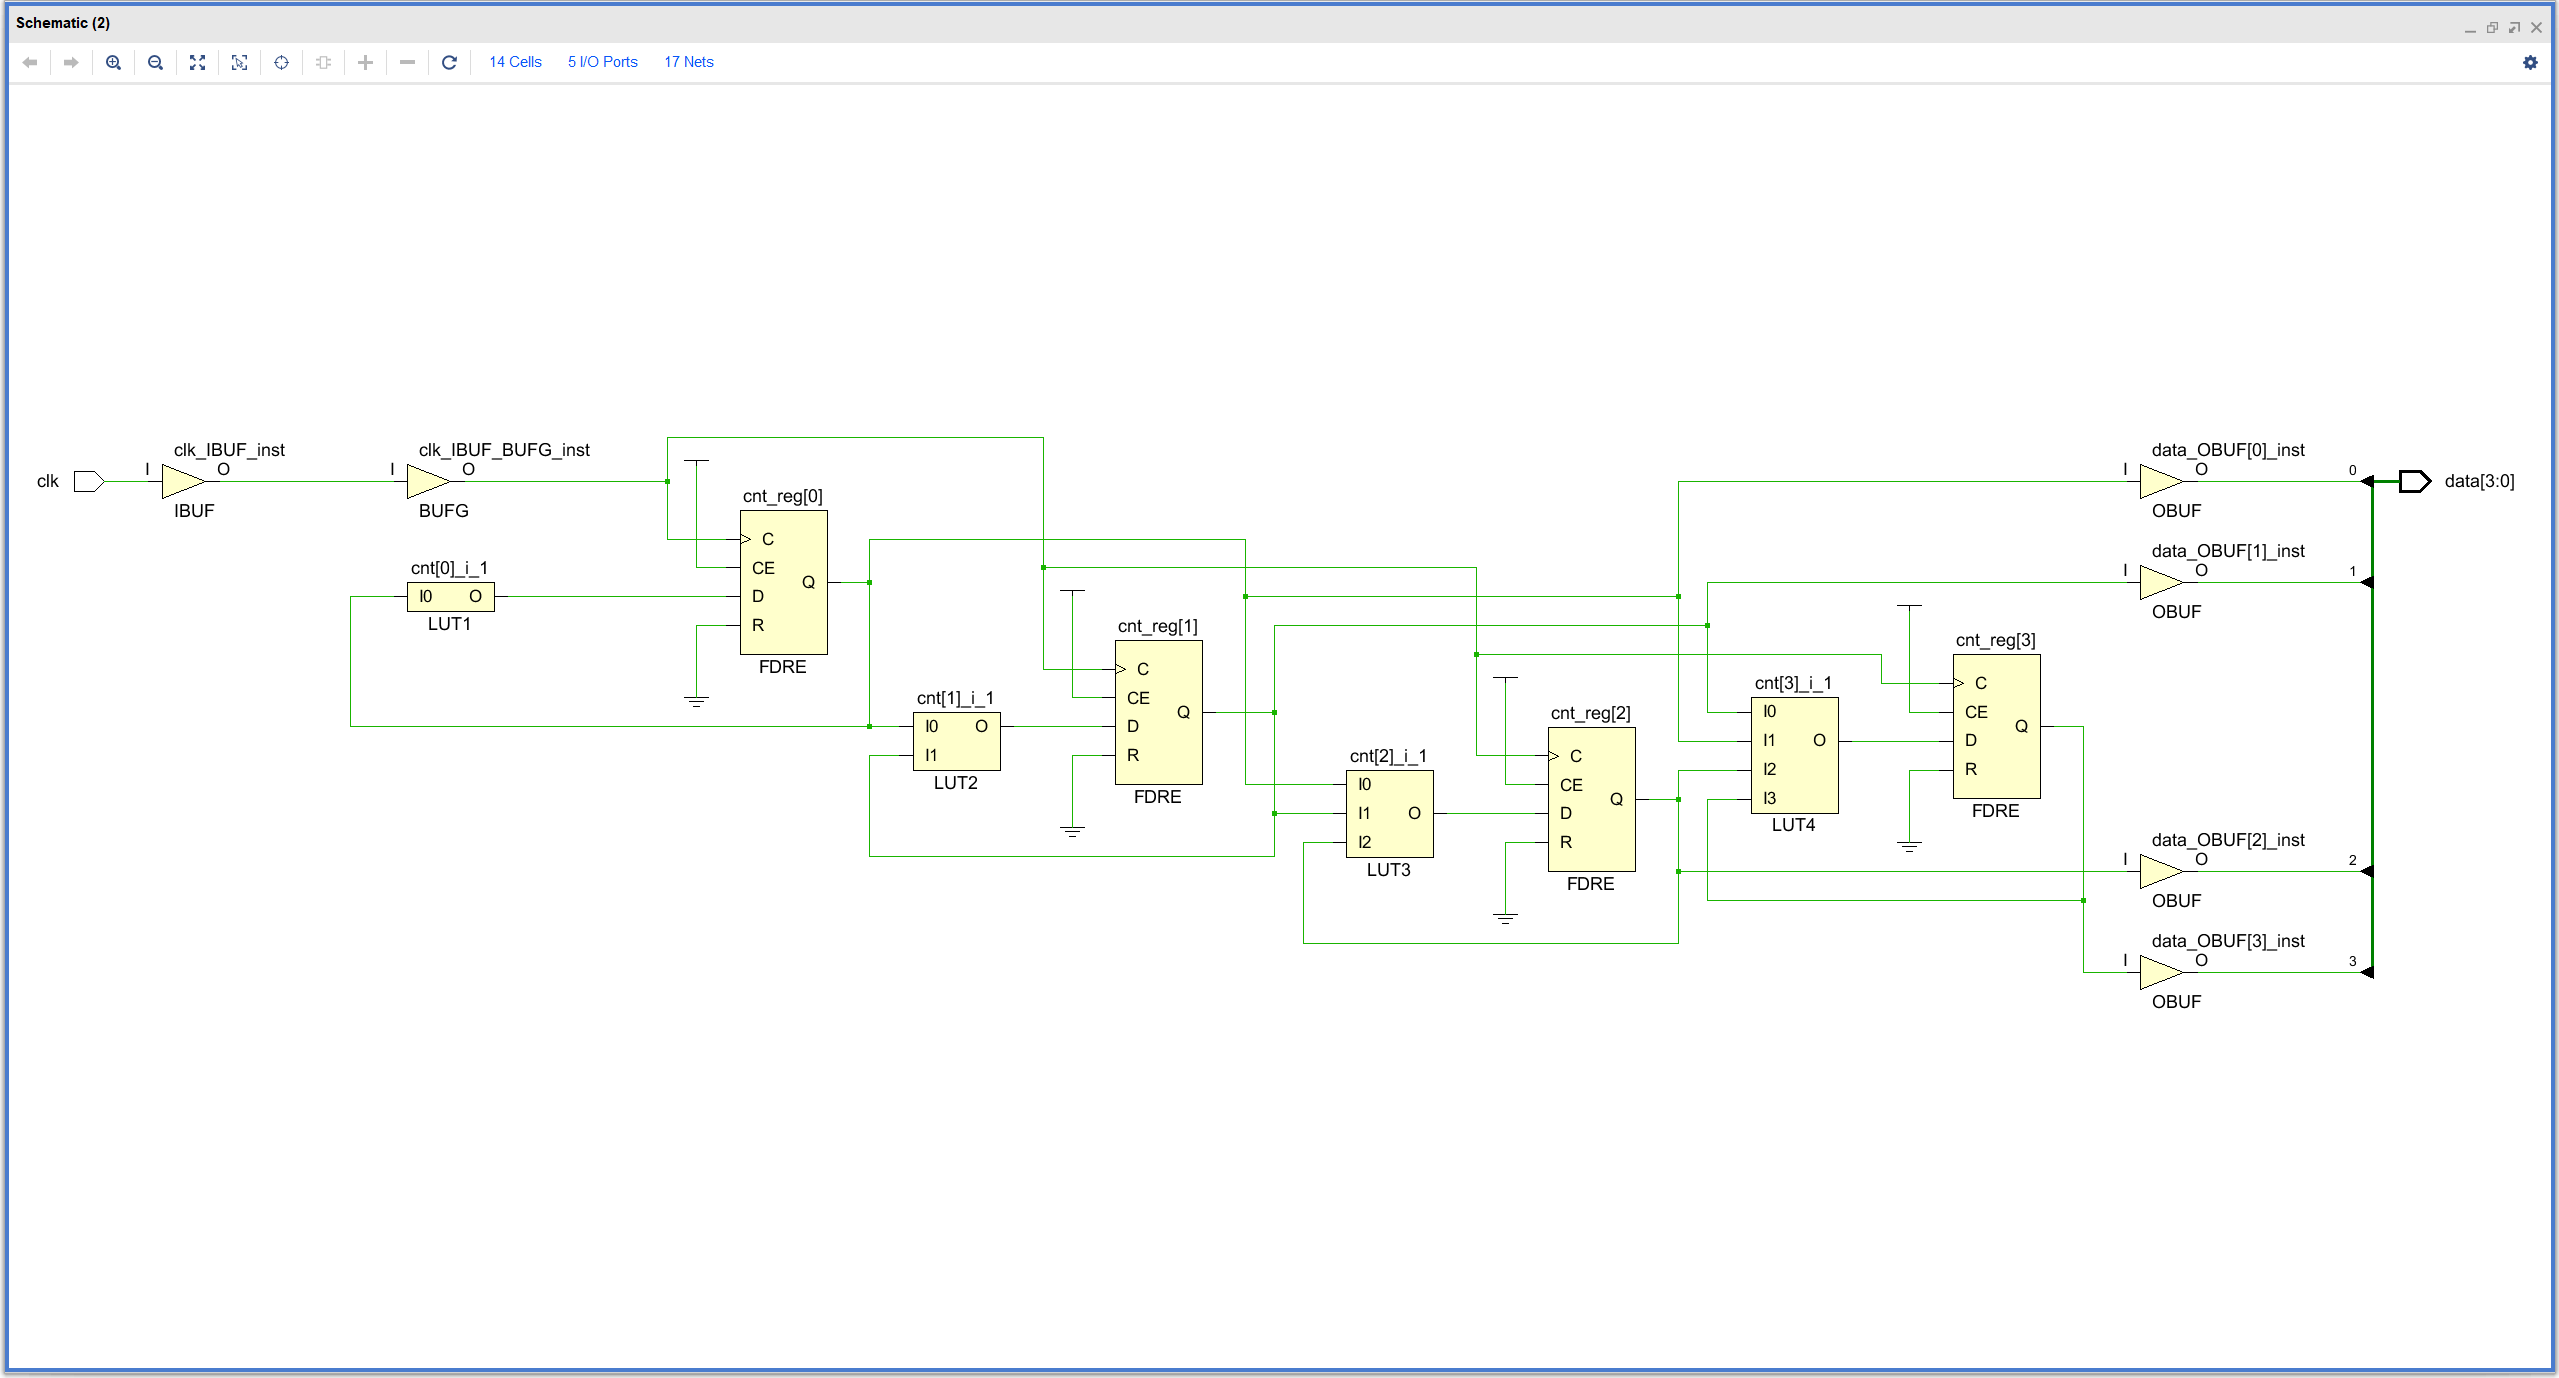
\includegraphics[width=0.3\textwidth]{nonex13.png}\par
在非阻塞控件中,所有控件操作在时钟上升沿时几乎同时触发,但值会在下一次更新时才生\par
一个时钟周期后,cnt = 1\par
两个时钟周期后,cnt = 2\par

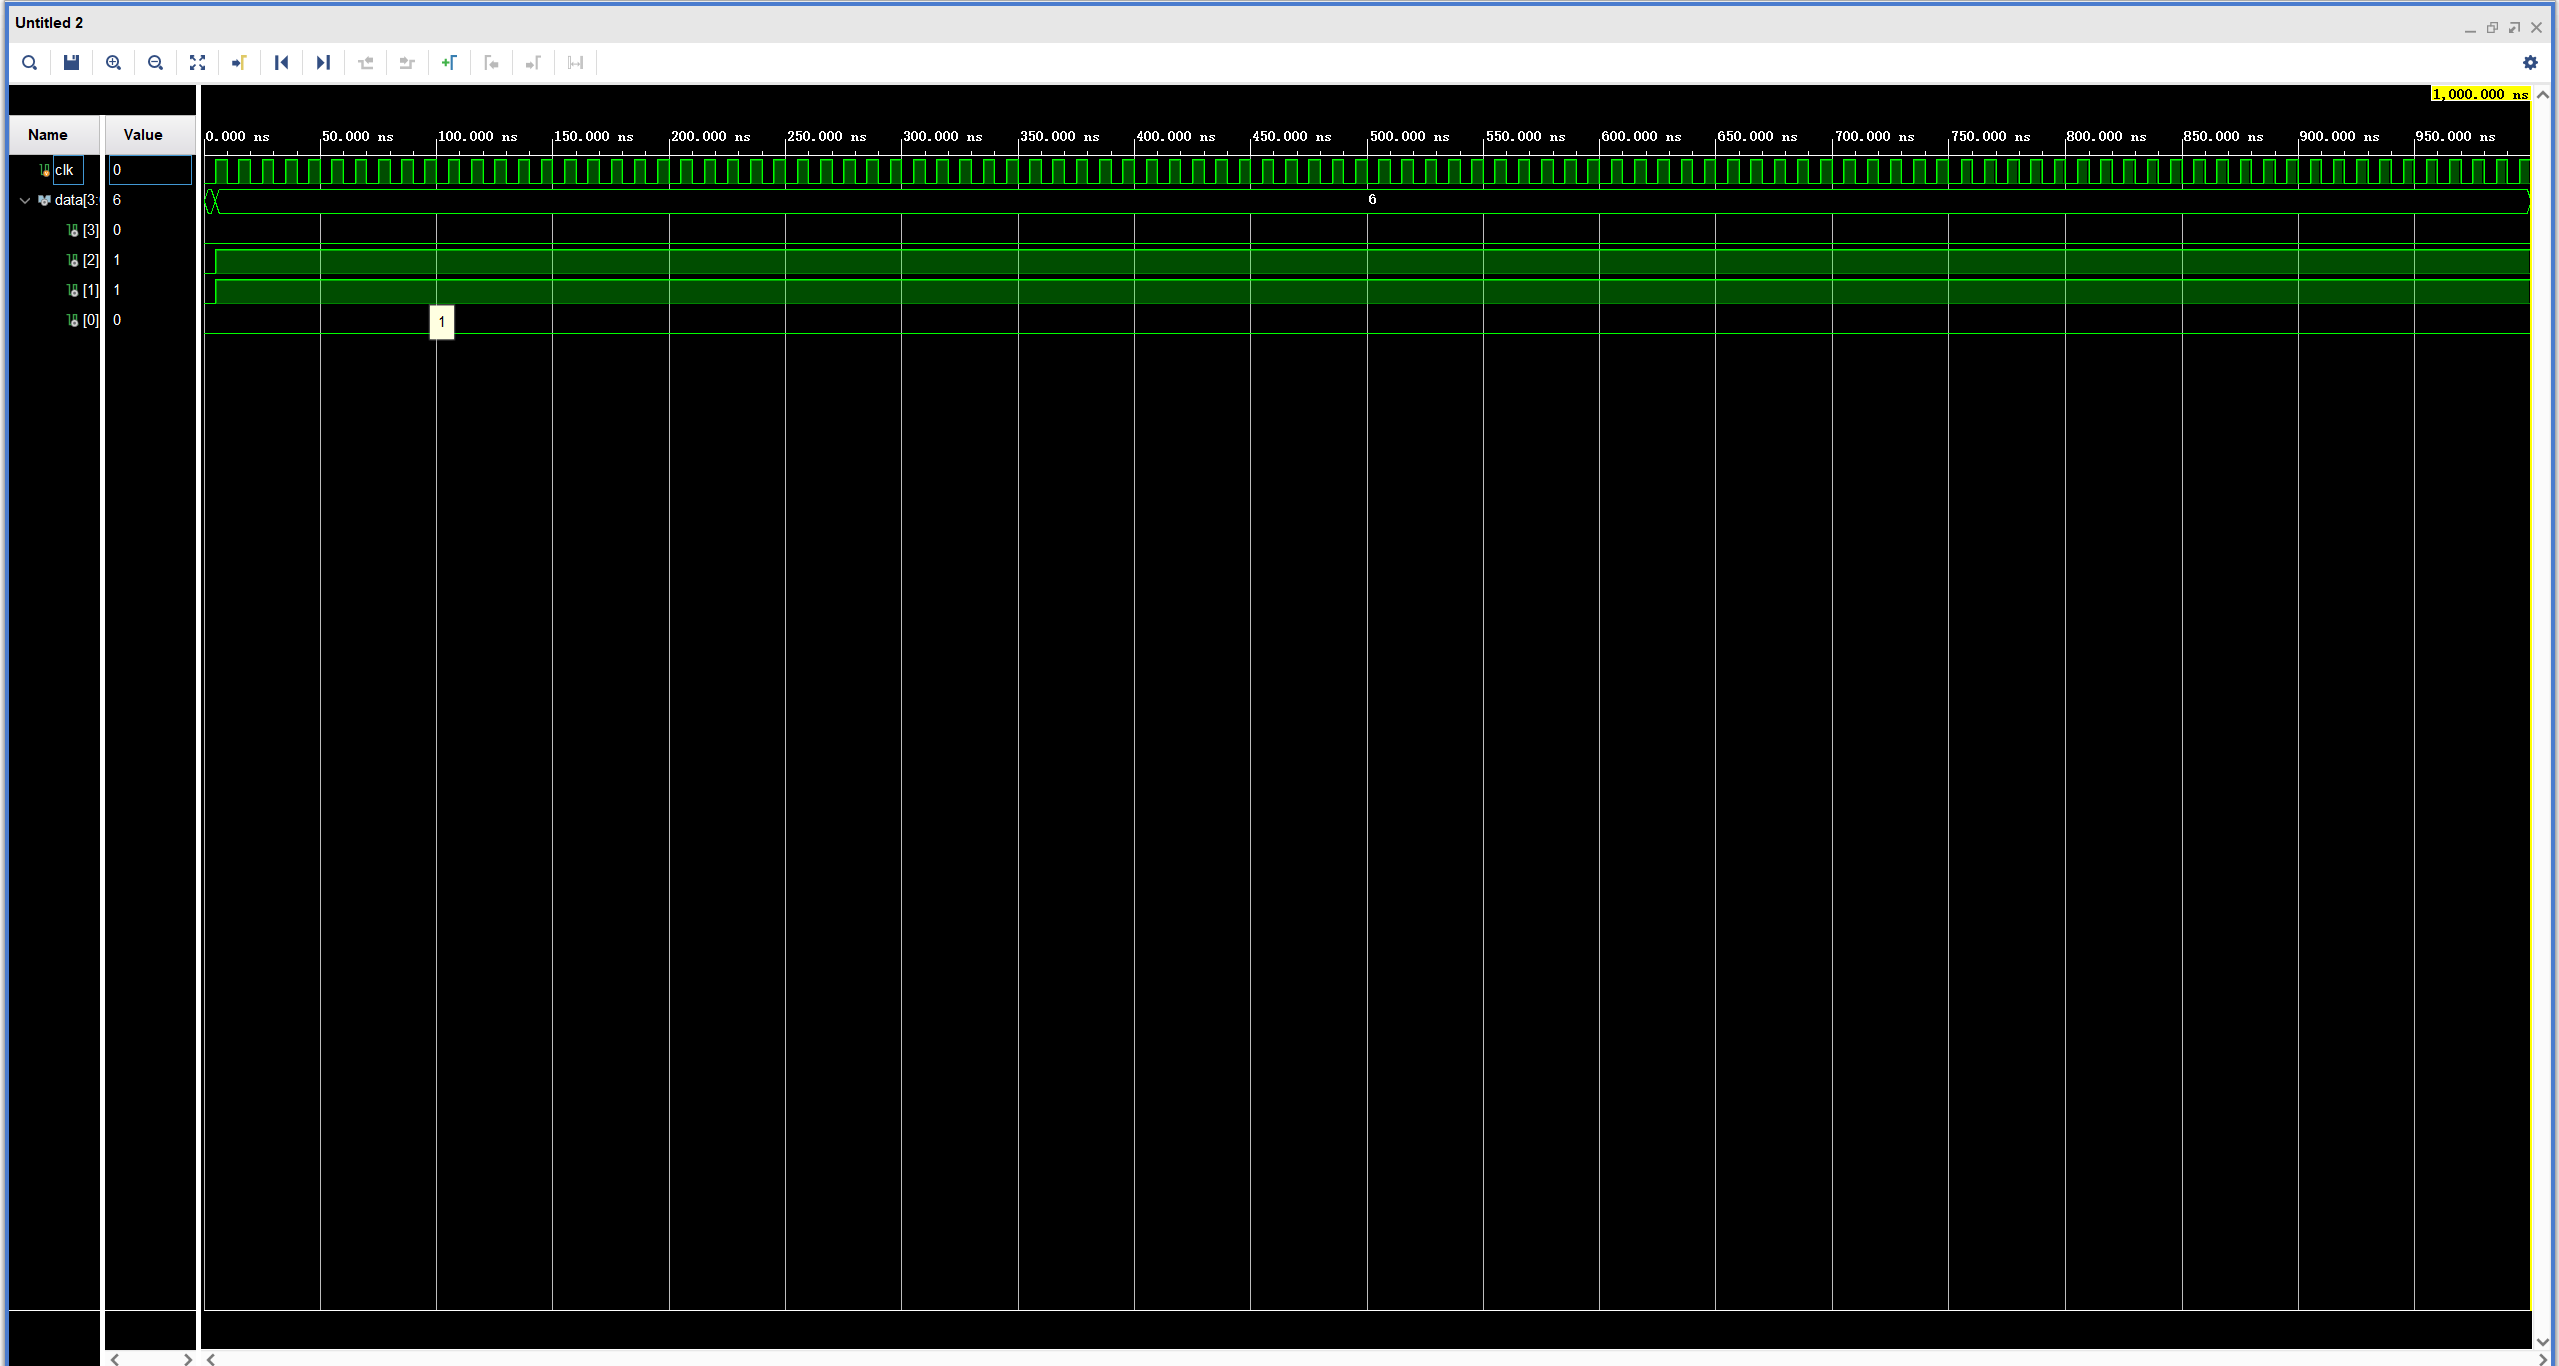
\includegraphics[width=0.3\textwidth]{ex11.png}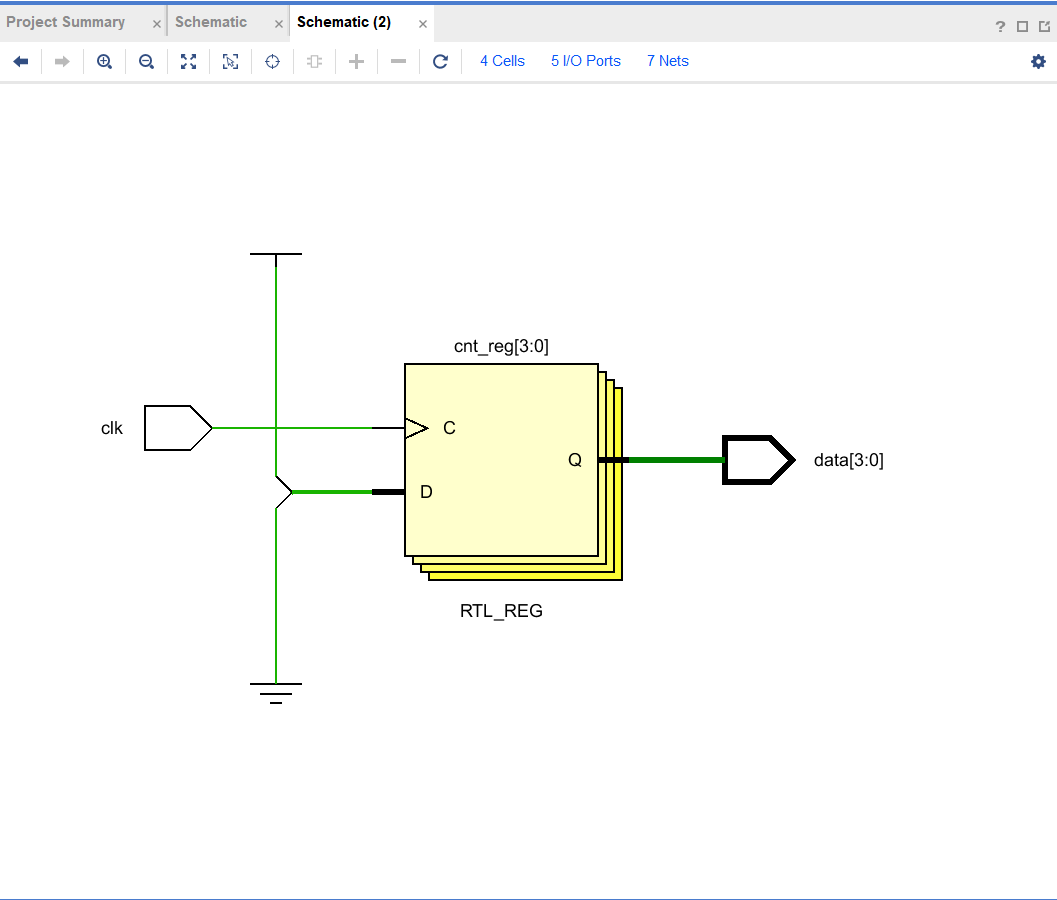
\includegraphics[width=0.3\textwidth]{ex12.png}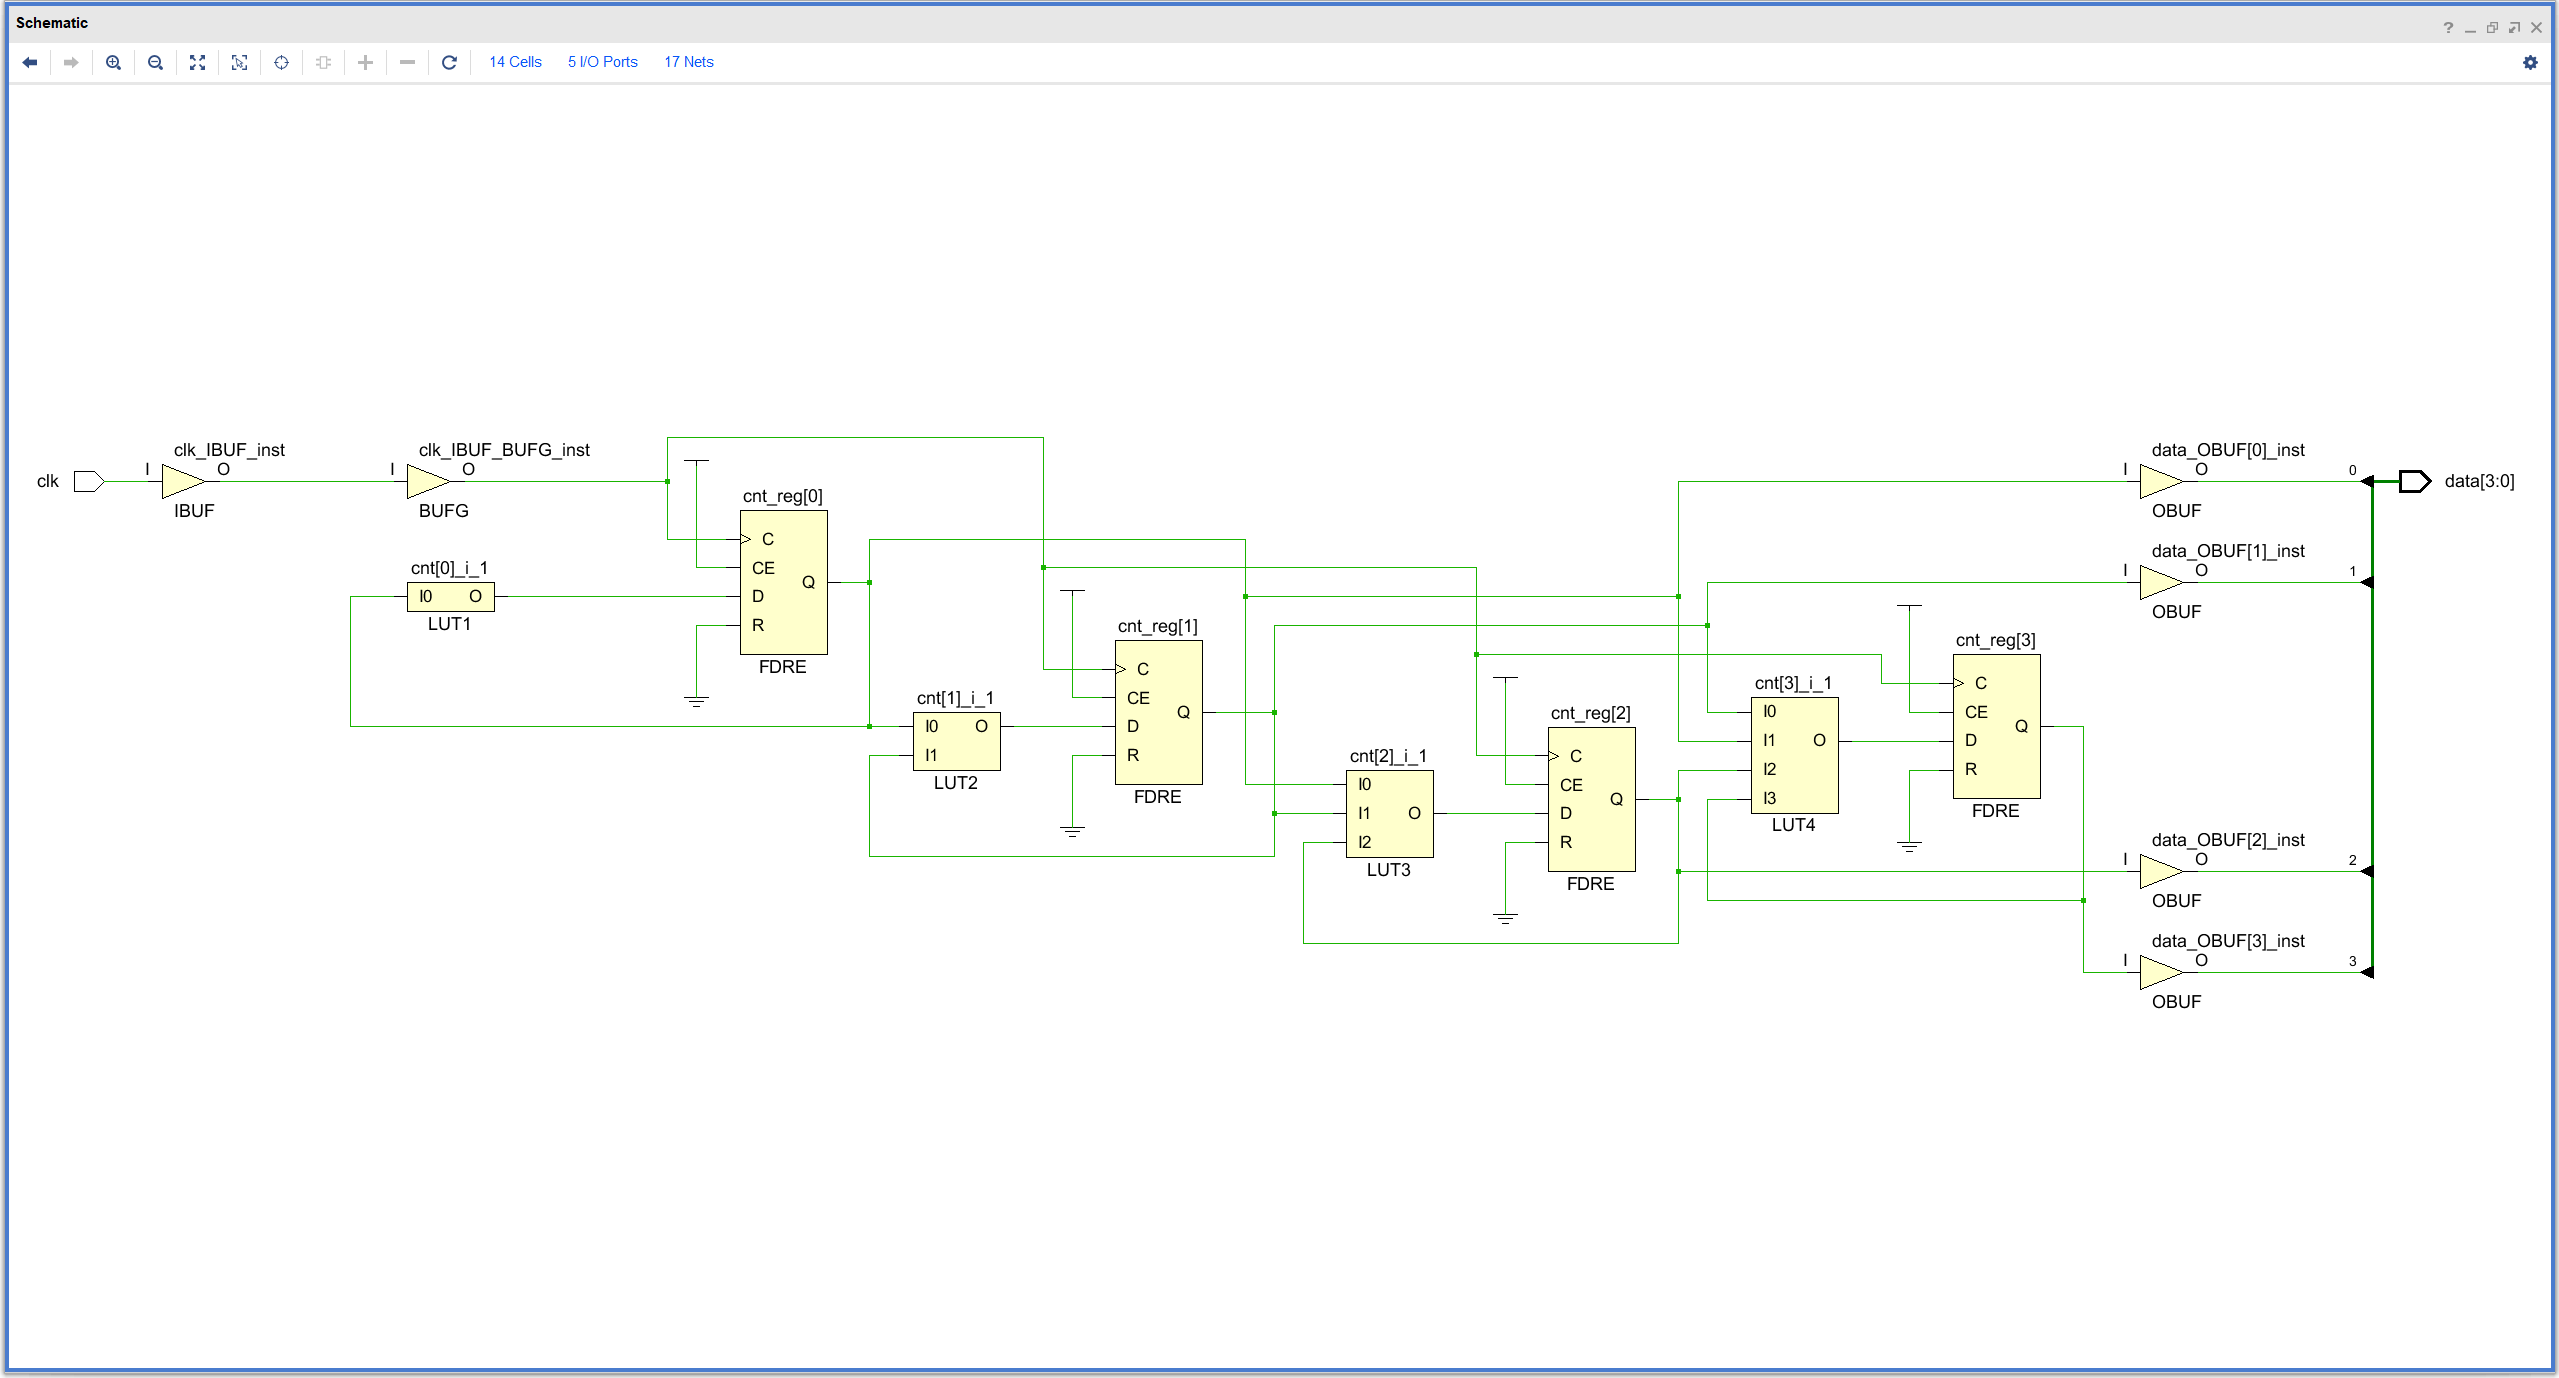
\includegraphics[width=0.3\textwidth]{ex13.png}\par
阻塞赋值是顺序执行的,即每条赋值语句都会在执行过程中立即更新变量的值\par
一个时钟周期后,cnt = 6。\par
两个时钟周期后,cnt = 6。\par

$$
$$
对比2\par
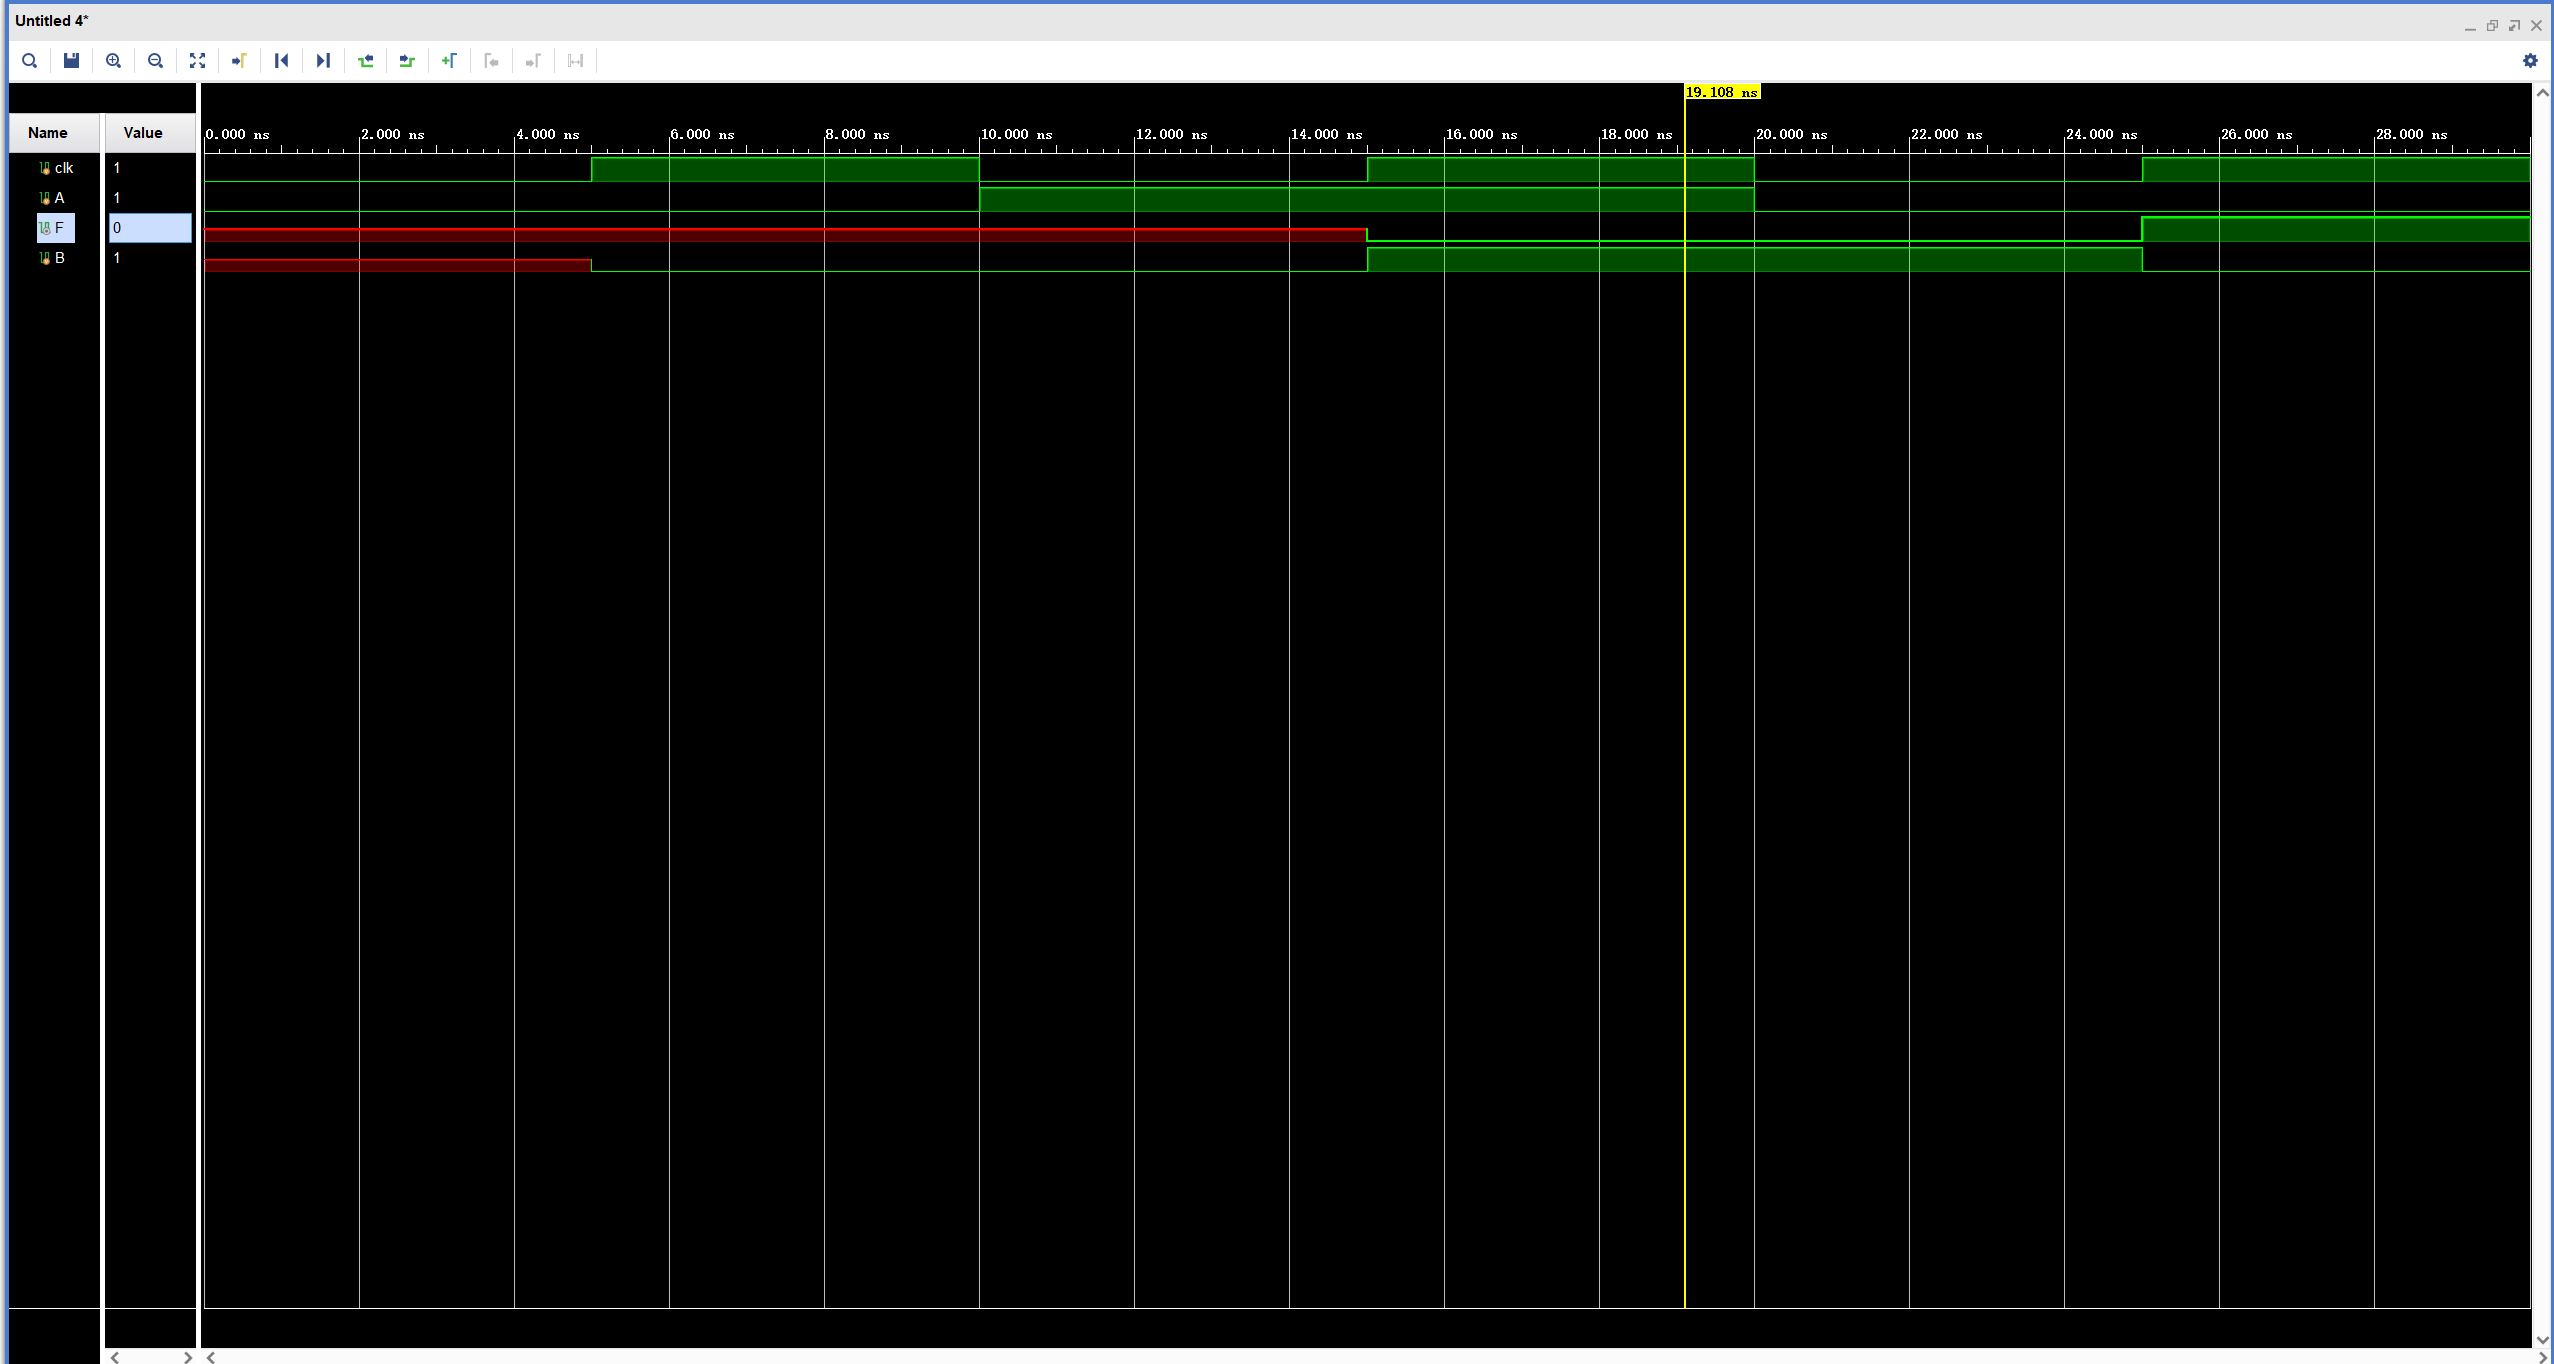
\includegraphics[width=0.3\textwidth]{nonex21.png}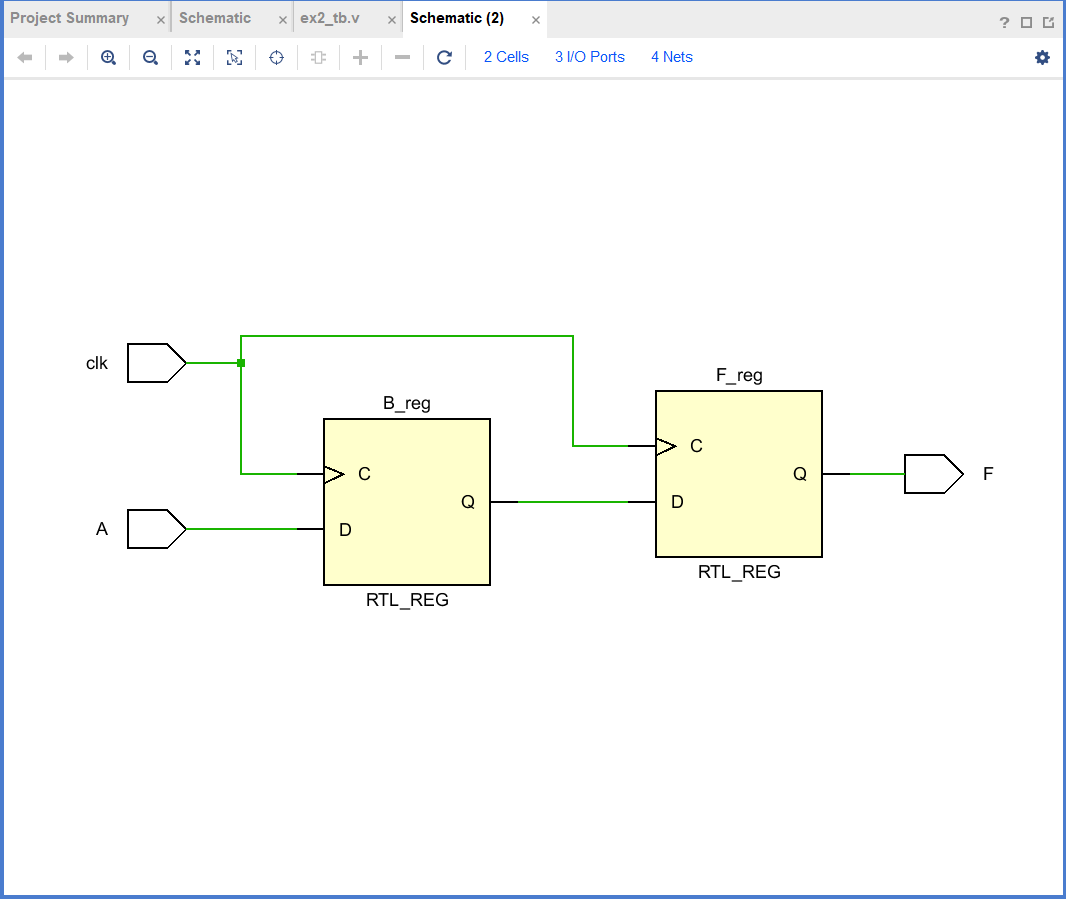
\includegraphics[width=0.3\textwidth]{nonex22.png}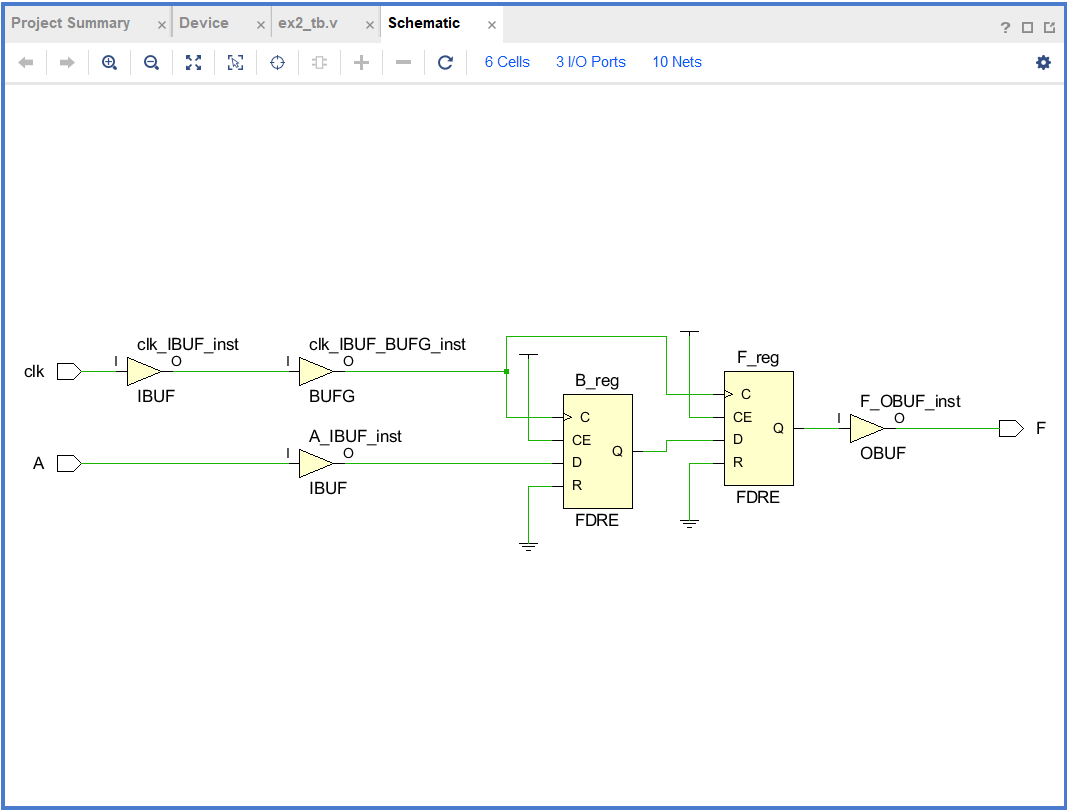
\includegraphics[width=0.3\textwidth]{nonex23.png}\par
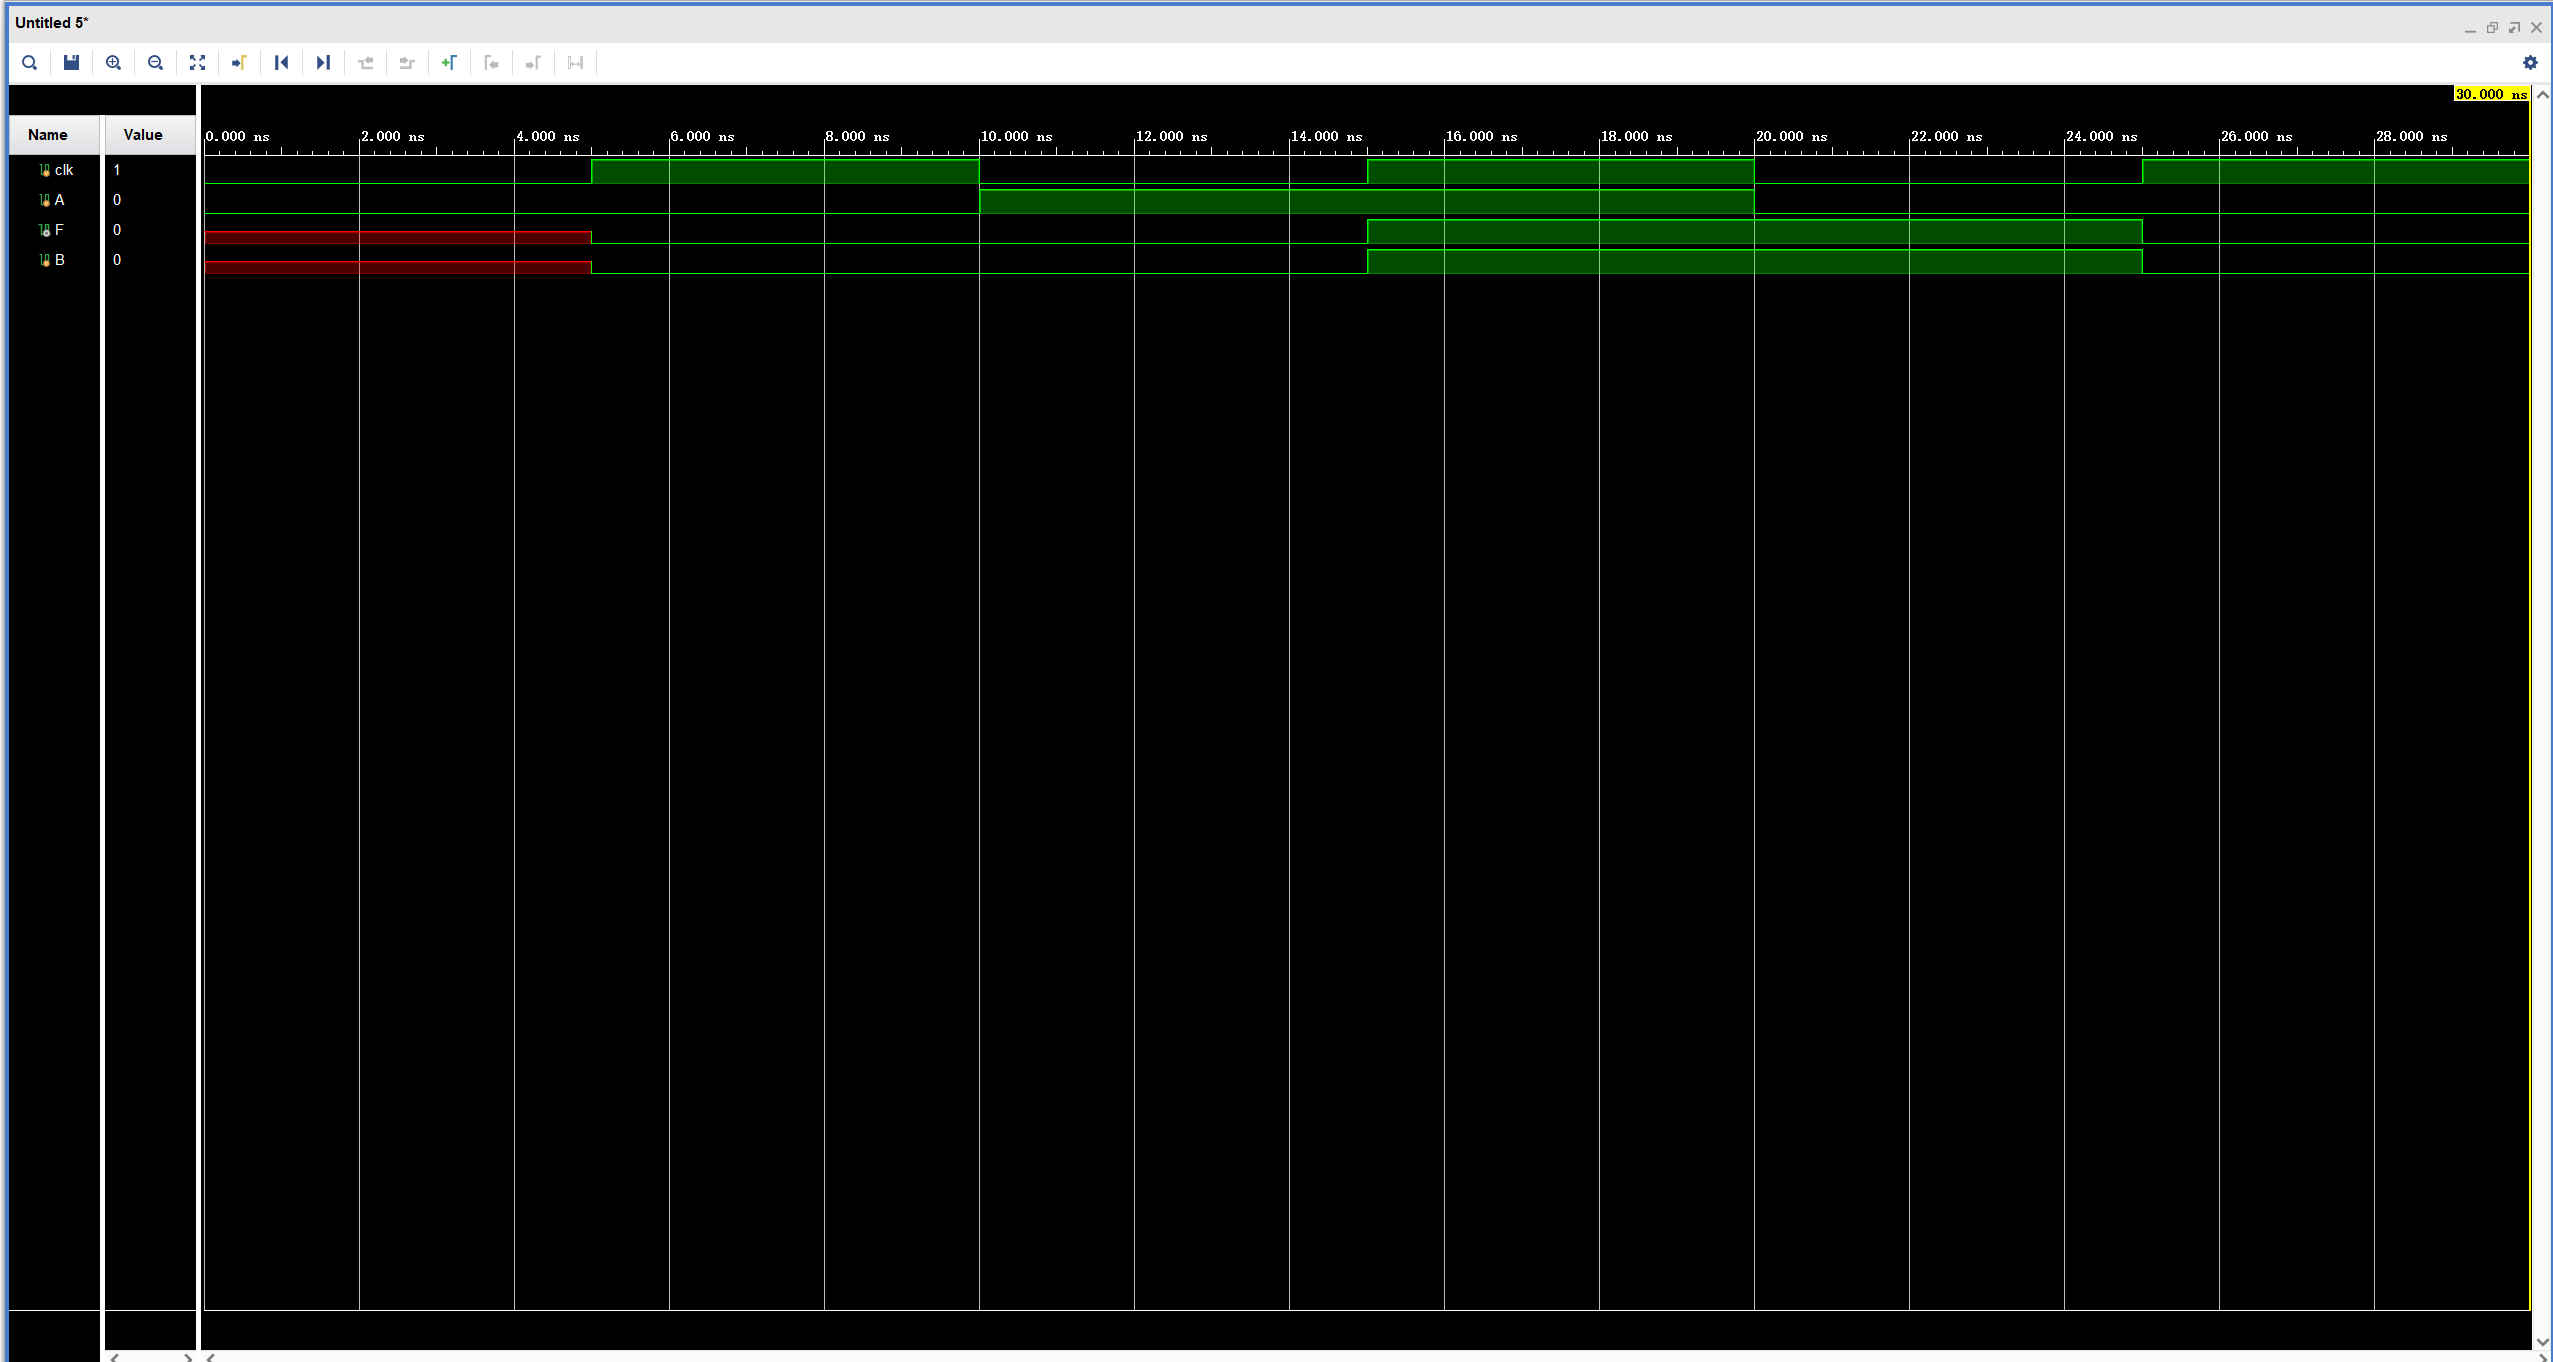
\includegraphics[width=0.3\textwidth]{ex21.png}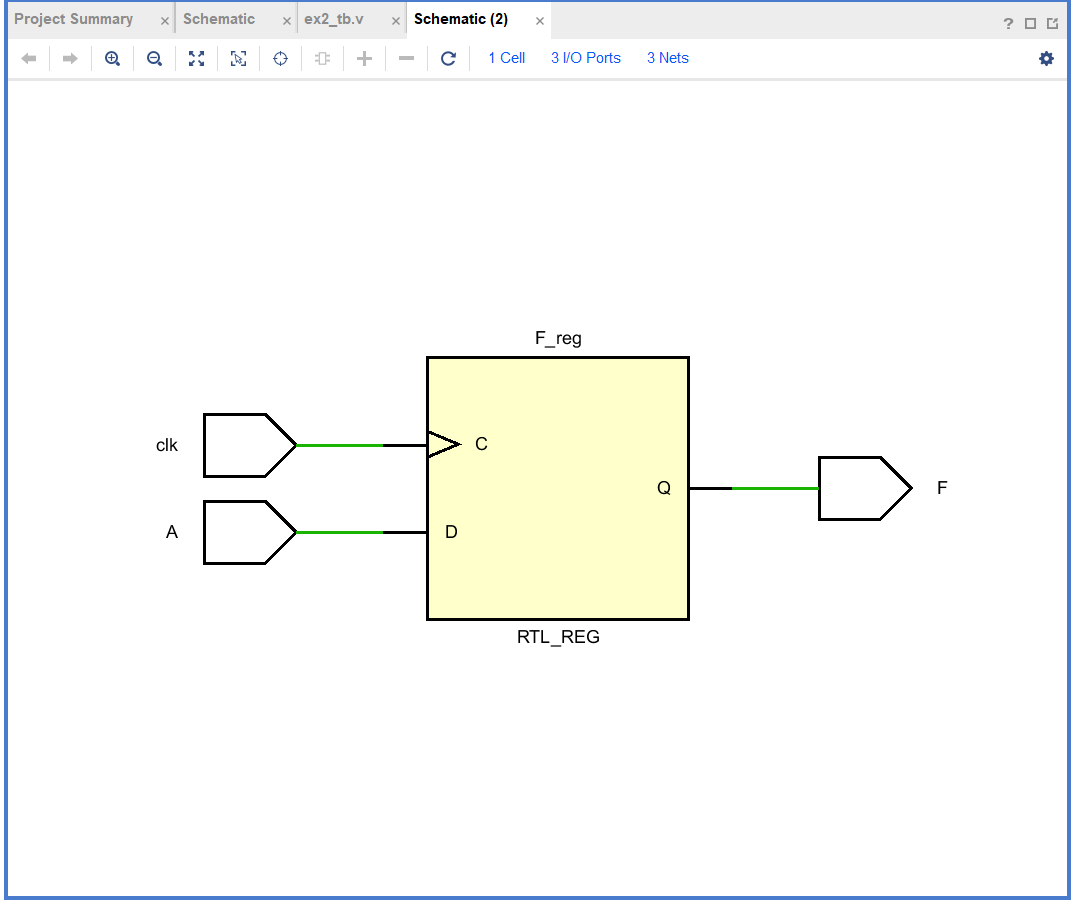
\includegraphics[width=0.3\textwidth]{ex22.png}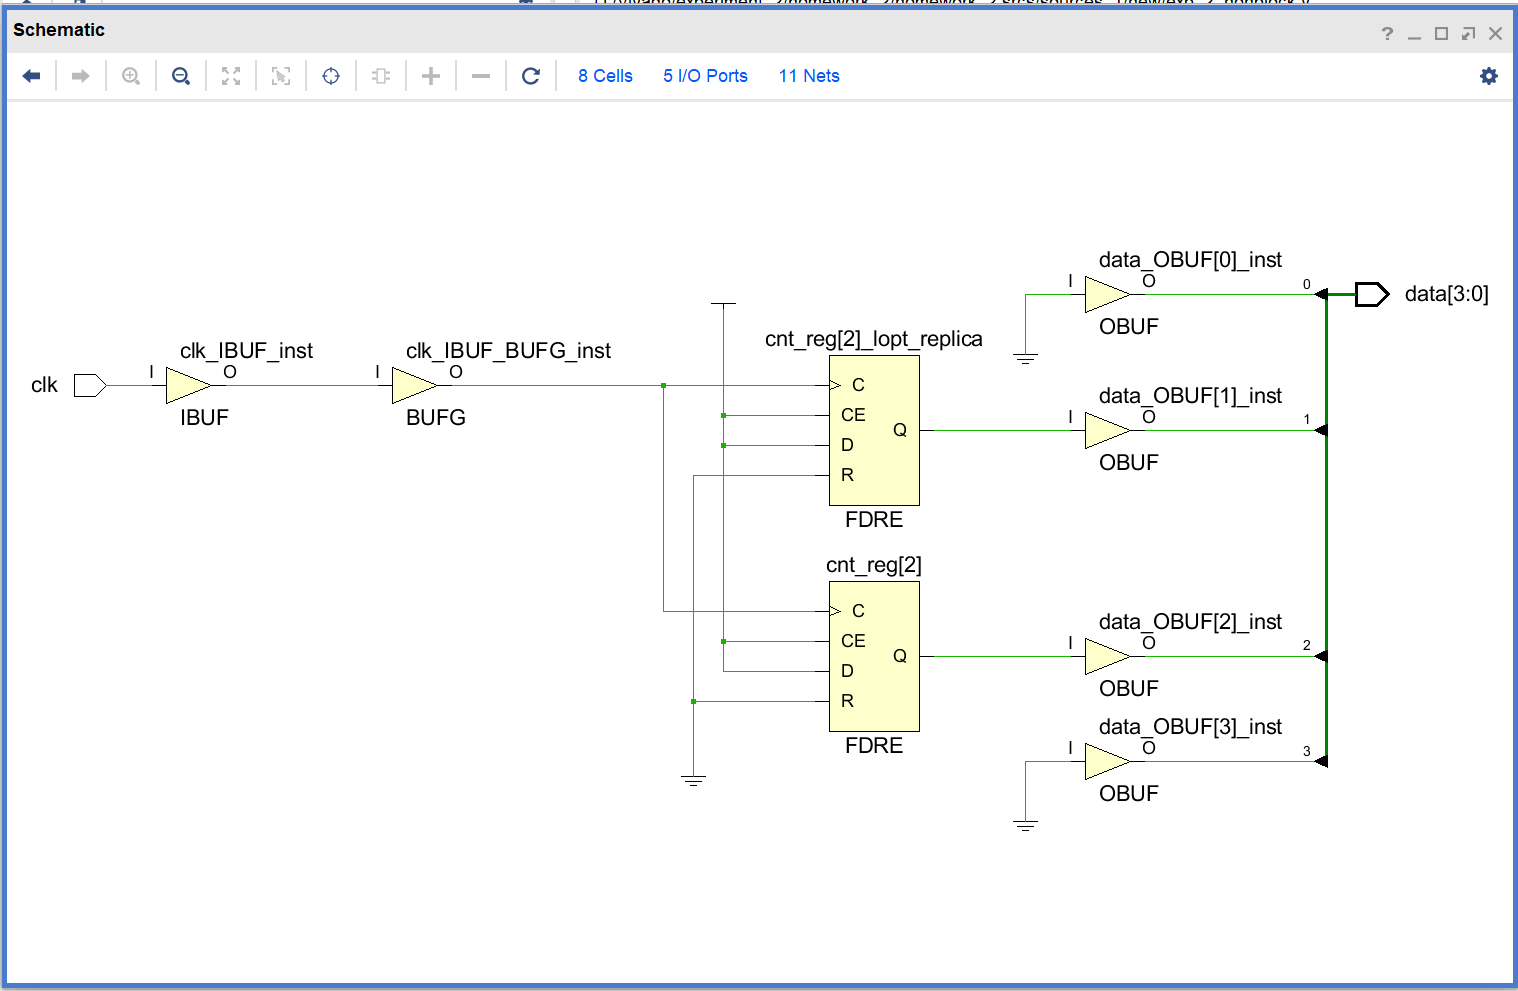
\includegraphics[width=0.3\textwidth]{new.png}\par
$$
$$
RTL图分析\par
非阻塞赋值( <=):\par
阻塞非赋值会触发控件操作,导致每次cnt <= 5和cnt <= cnt + 1'b1基于未更新的cnt值遭受损坏。\par
阻塞值 ( =):\par
阻塞赋值会按顺序依次执行。在同一个时钟周期内,cnt = 5会改变cnt当前的值,然后cnt = cnt + 1'b1根据更新后的cnt值进行侵犯。\par
综合电路图分析\par
非阻塞赋值( <=):\par
阻塞非阻塞通常会产生多级触发结构,每个非阻塞会生成一个独立的触发。\par
阻塞值 ( =):\par
阻止描述符的赋值是顺序执行的,可能会获取简单的组合逻辑或多个寄存器。\par


\end{document}